\documentclass[12pt,UTF8]{ctexart} % 使用ctexart文档类,UTF8编码,字体大小为12pt

% 中文与排版
\usepackage{ctex}
\usepackage{geometry}
\geometry{a4paper, left=2cm,right=2cm,top=2cm,bottom=2cm} % 页边距设置
\usepackage{pdfpages}

% 数学与符号
\usepackage{amsmath, amssymb, mathtools} % 数学公式与符号支持
\everymath{\displaystyle}
\usepackage{multicol}
\usepackage{enumitem}
%引用上标显示
\usepackage{subcaption}

\let\oldcite\cite
\renewcommand{\cite}[1]{\textsuperscript{\oldcite{#1}}}


% 定义choices环境
\newlist{choices}{enumerate}{1}
%\setlist[choices,1]{
	%	label=\Alph*.,
	%	leftmargin=2em,
	%	itemsep=0.3em,
	%	topsep=0.3em
	%}
\setlist[choices,1]{label=\Alph*., leftmargin=1.5em, itemsep=0em, before=\begin{multicols}{2}, after=\end{multicols}}
\usepackage{multicol}



% 图形与绘图
\usepackage{graphicx}
\usepackage{tikz}
\usetikzlibrary{arrows.meta}

% 列表与枚举
\usepackage{enumitem}
\setlist[enumerate,1]{label=\arabic*.}

% 表格
\usepackage{booktabs}
\usepackage{multirow}
\usepackage{array}

% 附录与浮动体
\usepackage{appendix}
\usepackage{float}

% 颜色与高亮
\usepackage{xcolor}
\usepackage{tcolorbox}
\definecolor{dkgreen}{rgb}{0,0.6,0}
\definecolor{gray}{rgb}{0.5,0.5,0.5}
\definecolor{mauve}{rgb}{0.58,0,0.82}
\definecolor{orange}{RGB}{255,127,0}

% 代码环境
\usepackage{listings}
\lstset{
	frame=tb,
	aboveskip=2mm,
	belowskip=2mm,
	showstringspaces=false,
	columns=flexible,
	framerule=1pt,
	rulecolor=\color{gray!35},
	backgroundcolor=\color{gray!5},
	basicstyle={\footnotesize\ttfamily\baselineskip=0.9\baselineskip},
	keywordstyle=\color{blue},
	commentstyle=\color{dkgreen},
	stringstyle=\color{mauve},
	breaklines=true,
	breakatwhitespace=true,
	tabsize=4,
	numbers=left,
	numberstyle=\scriptsize,
	stepnumber=1,
	lineskip=-1pt,
}


% 标题与超链接
\usepackage[breaklinks,colorlinks,bookmarksnumbered,linkcolor=black,urlcolor=blue]{hyperref}

% 段落与行距
\usepackage{indentfirst}
\setlength{\parindent}{2em}
\usepackage{setspace}
\renewcommand{\baselinestretch}{1.625}

% 目录深度设置
\setcounter{tocdepth}{4}
\setcounter{secnumdepth}{4}

\title{做题总结123}
\author{计算机专业 \\ perper}
\date{\today}

\begin{document}
%封面cover
\maketitle
\begin{figure}[H]
	\centering
	
\includegraphics[width=0.5\textwidth]{figure/xcpclogo.png} 
	%\caption{\textbf{插图测试}}
	\label{fig:logo}
\end{figure}
\newpage


%插入任意的pdf文件
%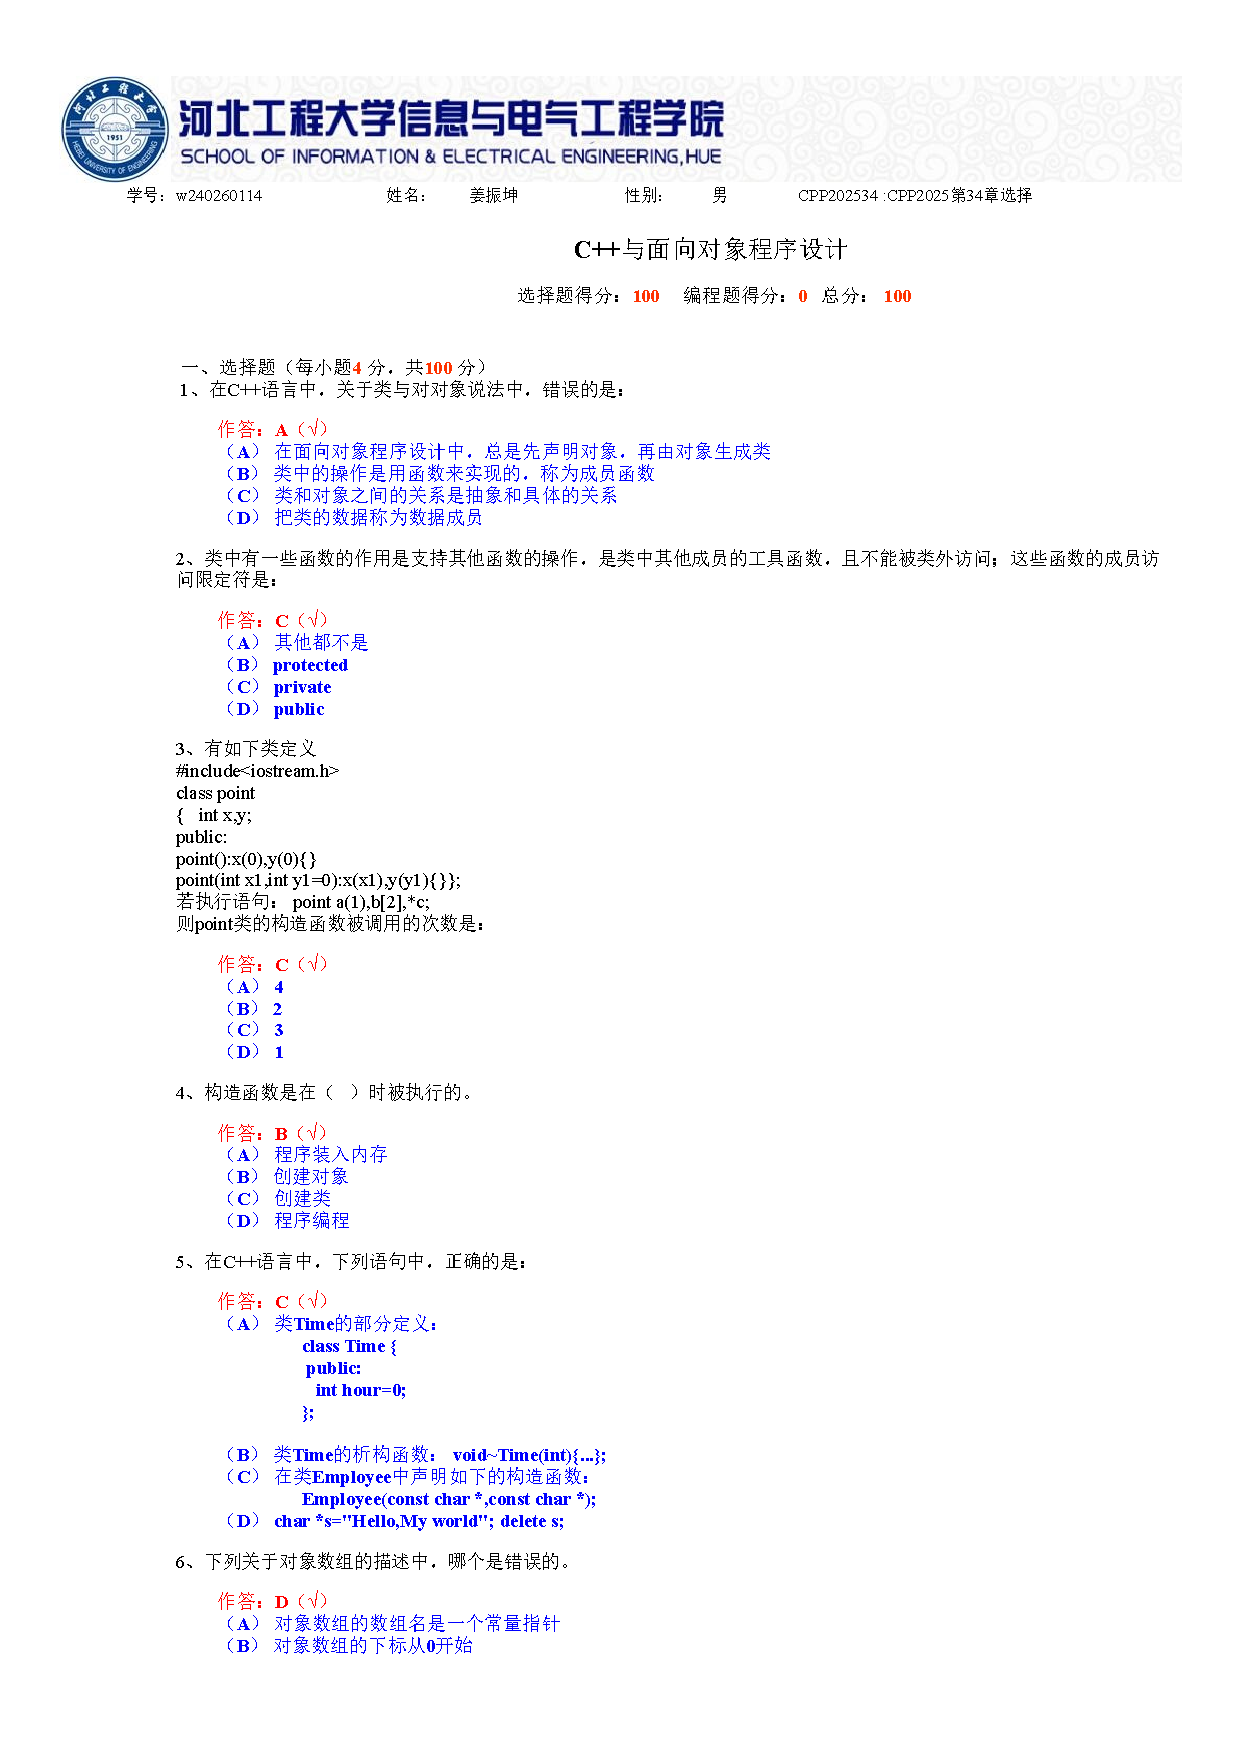
\includepdf{pdf/testpdf.pdf}


\tableofcontents

\newpage

\section{Codeforces 刷题总结}
%\textcolor{blue}{\textbf{271A}}
%\begin{lstlisting}[language=C++]\end{lstlisting}
在本节中，我将总结我在 Codeforces 上做题的经验。

\subsection{遇到的问题以及学到的方法}
\begin{itemize}
	\subsection{完美的一年}
	\item 题目链接：\href{https://codeforces.com/problemset/problem/271/A}{217A(点击此处)};方法:在判断一个字符串是否每个字符均不相等时可以用\textcolor{red}{set集合来去重}，\textcolor{red}{最终比较set的长度和原字符串的长度}来判断是非满足条件；
	
	代码示例：\\
\begin{lstlisting}[language=C++]
void solve() {
	ll n, num;
	cin >> n;
	num = n + 1;
	while (num) {
		string s;
		s = to_string(num);
		set<char> st(s.begin(), s.end());
		if (s.size() == st.size()) {
			cout << s << endl;
			break;
		}
		num++;
	}
}
\end{lstlisting}
\subsection{学校排队(与LuoguP3741类似)}
\item 题目链接:\href{https://codeforces.com/problemset/problem/266/B}{266B学校排队(点击此处)}；总结：通过字符串交换来达到目的的题都可以\textcolor{red}{用X填充思想；}
	
代码示例：\\
\begin{lstlisting}[language=C++]
void solve() {
	ll n, t;
	cin >> n >> t;
	string s1, s2;
	cin >> s1;
	s2 = s1;
	while (t--) {
		for (ll i = 0; i < n - 1; i++) {
			if (s1[i] == 'B' && s1[i + 1] == 'G' && s2[i] != 'X') {
				swap(s1[i], s1[i+1]);
				s2[i] = 'X';
				s2[i + 1] = 'X';
			}
		}
		s2=s1;
	}
	cout << s1 << endl;
}
\end{lstlisting}
\subsection{向上取整问题，不用ceil函数}
\item 题目链接：\href{https://codeforces.com/contest/1328/problem/A}{629A整除性问题(点击此处)}；

代码示例：\\
\begin{lstlisting}[language=C++]
void solve() {
	ll a, b;
	cin >> a >> b;
	if (a % b == 0) {
		cout << 0 << endl;
	} else {
		ll c = (a + b - 1) / b;//代替ceil函数实现向上取整即(a+b-1)/b
		ll d = c * b;
		cout << d - a << endl;
	}
}
\end{lstlisting}
\end{itemize}
\newpage
% \subsection{代码示例}
% 下面是一个代码示例：

% \begin{lstlisting}[language=C++]
	% #include <bits/stdc++.h>
	% using namespace std;
	
	% int main() {
		%     cout << "Hello Codeforces!" << endl;
		%     return 0;
		% }
	% \end{lstlisting}

\section{newcode 刷题总结}
%\textcolor{blue}{\textbf{271A}}
%\begin{lstlisting}[language=C++]\end{lstlisting}
在本节中，我将总结我在 newcode 上做题的经验。

\subsection{遇到的问题以及学到的方法}
\begin{itemize}
\subsection{周赛119}
\item 题目链接：\href{https://ac.nowcoder.com/acm/contest/122724/B}{B(点击此处)};思路：直接最大的-最小的(但是要先排序)；
	
代码示例：\\
\begin{lstlisting}[language=C++]
void solve(){
	int n;
	cin>>n;B
	vector<int>a(n);
	for(int i=0;i<n;i++){
		cin>>a[i];
	}
	sort(a.begin(),a.end());
	cout<<a.back()-a.front()<<endl;
}
\end{lstlisting}
\item 题目链接：\href{https://ac.nowcoder.com/acm/contest/122724/C}{C(点击此处)};方法：当遇到数学问题找满足条件的数字时要学会\textcolor{red}{打表(先写一个计算机写一个简易的代码逐渐扩大范围找有没有什么规律)}；
	
代码示例：\\
\begin{lstlisting}[language=C++]
#include <bits/stdc++.h>
using namespace std;
int main(){
	int l,r;
	cin>>l>>r;
	for(int i=l;i<=r;i++){
		if(需要的条件){
			cout<<i<<endl;
		}
	}
}
\end{lstlisting}
最终发现不论在哪样大的范围里只有1和9满足条件；
\subsection{月赛124}
\subsubsection{B(数组重排)}
\item 题目链接：\href{https://ac.nowcoder.com/acm/contest/123787/B}{B数组重排(点击此处)}总结：因为i是逐渐递增的，所以只要数组逐渐递减就可以使元素减去下标的值互不相等；
	
代码示例：\\
\begin{lstlisting}[language=C++]
#include <bits/stdc++.h>
using namespace std;
using ll = long long;

int main() {
	ios::sync_with_stdio(false);
	cin.tie(nullptr);
	
	int T;
	if (!(cin >> T)) return 0;
	while (T--) {
		int n;
		cin >> n;
		vector<ll> a(n);
		for (int i = 0; i < n; ++i) cin >> a[i];
		sort(a.begin(), a.end(), greater<ll>()); // 降序排列
		for (int i = 0; i < n; ++i) {
			if (i) cout << ' ';
			cout << a[i];
		}
		cout << '\n';
	}
	return 0;
}

\end{lstlisting}
\subsubsection{D区间查询\textcolor{red}{(求因数模板)}}
\item 题目链接：\href{https://ac.nowcoder.com/acm/contest/123787/D}{D区间查询(点击此处)};

代码示例：\\
\begin{lstlisting}[language=C++]
void solve(){
	cin>>a>>b>>l>>r;
	ll d,ans=0;
	d=b-a;
	for(ll i=1;i*i<=d;++i){
		if(d%i==0){
			//因子i；
			ll x1=b+d/i;
			if(x1>=l&&x1<=r){
				ans++;
			}
			//因子d/i(与i成对);
			if(i*i!=d){  //避免重复
				ll x2=b+i;
				if(x2>=l&&x2<=r){
					ans++;
				}
			}
		}
	}
	cout<<ans<<endl;
}
\end{lstlisting}
\subsection{周赛121}
\subsubsection{B不想被吃掉}
\item 题目链接：\href{https://ac.nowcoder.com/acm/contest/124143/B}{B不想被吃掉(点击此处)}；总结：根据贪心可知，下一天最好先把上一天剩下的先吃完，因为上一天剩下的这天之后就不能吃了。

代码示例：\\
\begin{lstlisting}[language=C++]
void solve(){
	ll n,x;
	cin>>n>>x;
	vector<ll> v(n+1);
	for(ll i=1;i<=n;i++){
		cin>>v[i];
	}
	ll prev=0;
	for(ll i=1;i<=n;i++){
		ll use=min(prev,x); //先吃上一天剩下的。
		ll need=x-use; //计算吃掉上一天的后还需要多少。
		if(v[i]<need){
			cout<<"No"<<endl;
			return;
		}
		prev=v[i]-need;
	}
	cout<<"Yes"<<endl;
}
\end{lstlisting}
\subsubsection{查找符合条件字串(C三妖精say subsequence )}
\item 题目链接：\href{https://ac.nowcoder.com/acm/contest/124143/C}{C三妖精say subsequence}；

代码示例：\\
\begin{lstlisting}[language=C++]
void solve(){
	ll n;
	string s;
	cin>>n>>s;
	vector<ll> v(26);
	//计算每一个字母的个数实则是看看每个字母可以放几个位置，像数学里的全排列
	for(auto x:s){
		v[x-'a']++;
	}
	ll ans=0;
	//三个for循环的作用是保证三个字符两两不同
	for(ll i=0;i<26;i++){
		for(ll j=i+1;j<26;j++){
			for(ll k=j+1;k<26;k++){
				ans=(ans+v[i]*v[j]*v[k]*6)%MOD;//*6的意思是只有三个字符，
			}                   //每次对选出来的三个字符全排列的个数是6
		}
	}
	cout<<ans<<endl;
}
\end{lstlisting}
\subsubsection{D01串大冒险}
\item 题目链接：\href{https://ac.nowcoder.com/acm/contest/124143/D}{D恋恋的01串大冒险(点击此处)}；

代码示例：\\
\begin{lstlisting}[language=C++]
void solve(){
	ll n,k;
	string s;
	cin>>n>>k>>s;
	s=' '+s;
	ll cur_zero=0,i=1;
	ll cnt=0;
	while(i<=n){
		if(s[i]=='1'){
			if(i<=n&&s[i]=='1'){
				i++;
			}
			cur_zero=0;
		}else{
			cur_zero++;
			if(cur_zero==k){
				v[cnt++]=i-1;
				cur_zero=0;
			}
			i++;
		}
		if(i>n){
			v[cnt]=i-1;
			break;
		}
	}
	for(ll j=1;j<=n;j++){
		v[j]=max(v[j],v[j-1]);
	}
	for(ll j=0;j<=n;j++){
		cout<<v[j]<<" ";
	}
}
\end{lstlisting}
\subsection{周赛125}
\subsubsection{D小苯的01合并}
\item 题目链接：\href{https://ac.nowcoder.com/acm/contest/126319/D}{D小苯的01合并(点击此处)}；总结：用队列寻找字串是一个较为新颖的思想，可以学习一下。
\textcolor{orange}{变式题在AcWing2816};

代码示例：
\begin{lstlisting}[language=C++]
auto solve() -> void {
	ll n, m;
	cin >> n >> m;
	string s1, s2;
	cin >> s1 >> s2;
	queue<ll> q1, q2;
	for (ll i = 0; i < n; i++) {
		q1.emplace(s1[i] - '0');
	}
	for (ll i = 0; i < m; i++) {
		q2.emplace(s2[i] - '0');
	}
	while (q1.size() && q2.size()) {
		if (q1.front() == q2.front()) {
			q1.pop();
			q2.pop();
		} else {
			const ll x = q1.front();
			q1.pop();
			q1.front() ^= x;
		}
	}
	//0和任意数异或都等于那个数，所以最后如果剩下偶数个1或者若干个0时可以消掉；
	ll remain = 0;
	while (q1.size()) {
		remain ^= q1.front();
		q1.pop();
	}
	if (remain == 0 && q2.size() == 0) {
		cout << "YES" << endl;
	} else {
		cout << "NO" << endl;
	}
}
\end{lstlisting}
\subsection{每日一题}
\subsubsection{12.4质数统计(筛法列质数表)}
\item 题目链接：\href{https://www.nowcoder.com/practice/d832b0c1a0bd4394a3229f06c6f0b50b?channelPut=tracker2}{12.4质数统计(点击此处)}；用筛法先把所有质数列成一个表，然后直接查找；思想：若找到一个质数，那么就把它的倍数全部删掉；

代码示例：\\
\begin{lstlisting}[language=C++]
const int N=1e6+10;
ll d[N];
ll num[N];
void solve() {
	ll q;
	cin >> q;
	for (ll i = 2; i < N; ++i) {
		if (d[i] == 1)continue;
		num[i]++;
		for (ll j = i + i; j < N; j += i) {
			d[j] = 1;
		}
	}
	for (ll i = 1; i < N; ++i) {
		num[i] += num[i - 1];
	}
	while (q--) {
		ll l, r, cnt = 0;
		cin >> l >> r;
		cnt = num[r] - num[l - 1];
		cout << cnt << endl;
	}
}
\end{lstlisting}
\subsection{其他}
\subsubsection{括号配对}
\item 题目链接：\href{https://www.nowcoder.com/practice/57260c08eaa44feababd05b328b897d7?tpId=383&tqId=296645&sourceUrl=%2Fexam%2Foj%2Fta%3FtpId%3D383%26channelPut%3Dacbanner25}{noob84括号配对问题(点击此处)}；
用栈进行；

代码示例：\\
\begin{lstlisting}[language=C++]
#include <bits/stdc++.h>
using namespace std;

int main() {
	string s;
	cin >> s;
	int n = s.size();
	stack<char> st;
	int b = 1;
	for (int i = 0; i < n; i++) {
		if (s[i] == '(' || s[i] == '[') {
			st.push(s[i]);
		} else if (s[i] == ']') {
			if (st.empty() || st.top() != '[') {
				b = 0;
				break;
			}
			st.pop();
		} else if (s[i] == ')') {
			if (st.empty() || st.top() != '(') {
				b = 0;
				break;
			}
			st.pop();
		}
	}
	if (b)cout << "true" << endl;
	else cout << "false" << endl;
	return 0;
}
\end{lstlisting}
\subsubsection{map里面套map的用法}
\item 题目链接：\href{https://ac.nowcoder.com/acm/contest/125954/C}{周赛123C小红出对(点击此处)}\\\textcolor{red}{下面这种遍历方法非常重要，一定要会用！！！}；

代码示例：\\
\begin{lstlisting}[language=C++]
auto solve() -> void {
	ll n;
	cin >> n;
	map<ll, map<char, ll> > mp;
	for (ll i = 1; i <= n; i++) {
		ll num;
		char c;
		cin >> num >> c;
		if (mp[num].find(c) == mp[num].end()) {
			mp[num][c] = i;
		}
	}
	vector<pair<ll, ll> > v;
	//一定要理解下面这种遍历方式和在这题中的技巧性。
	for (auto &[num,ch]: mp) {
		vector<ll> dis;
		for (auto &[c,id]: ch) {
			dis.push_back(id);
		}
		for (ll i = 0; i + 1 < dis.size(); i += 2) {
			v.push_back({dis[i], dis[i + 1]});
		}
	}
	cout << v.size() * 2 << endl;
	for (auto x: v) {
		cout << x.first << " " << x.second << endl;
	}
}
\end{lstlisting}
\subsubsection{BGN18 回文日期}
\item 题目链接：\href{https://www.nowcoder.com/practice/0372242deac541d0b578cc6563395681?tpId=385&tags=&title=&difficulty=0&judgeStatus=0&rp=0&sourceUrl=%2Fexam%2Foj%3FquestionJobId%3D10%26subTabName%3Donline_coding_page}{回文日期(点击此处)}；

代码示例：\\
\begin{lstlisting}[language=C++]
// 月份天数表，平年情况
int days[13] = {0, 31, 28, 31, 30, 31, 30, 31, 31, 30, 31, 30, 31};

// 检查日期是否合法
bool check(int date) {
	int year = date / 10000;
	int month = date % 10000 / 100;
	int day = date % 100;
	
	if (month == 0 || month > 12) return false;
	if (day == 0) return false;
	
	// 针对 2 月处理闰年
	if (month != 2) {
		if (day > days[month]) return false;
	} else {
		bool leap = (year % 4 == 0 && year % 100 != 0) || (year % 400 == 0);
		if (day > 28 + leap) return false;
	}
	return true;
}

int main() {
	int date1, date2;
	cin >> date1 >> date2;
	
	int ans = 0;
	// 策略：枚举年份（前四位）
	for (int i = 1000; i <= 9999; i++) {
		// 构建回文：把 i 翻转作为后四位
		// 例如 i = 2021, t = 1202
		int t = i, date = i;
		for (int j = 0; j < 4; j++) {
			date = date * 10 + t % 10;
			t /= 10;
		}
		
		// 判断构造出的日期是否在范围内，且日期本身合法
		if (date >= date1 && date <= date2 && check(date)) {
			ans++;
		}
	}
	
	cout << ans << endl;
	return 0;
}
\end{lstlisting}
\textcolor{red}{总结：要是从其实日期一直遍历到终止日期太过复杂要考虑闰年还有年份天数等多种情况，所以我们就选择遍历所有年份看看对应回文串的日期和天数是否合法即可}：要多培养逆向思维！！！

\subsubsection{BGN24 小红的矩阵染色}
\item 题目链接：\href{https://www.nowcoder.com/practice/f8b771318bb04490b7389cc35e148166?tpId=385&tags=&title=&difficulty=0&judgeStatus=0&rp=0&sourceUrl=%2Fexam%2Foj%3Fpage%3D1%26tab%3D%25E7%25AE%2597%25E6%25B3%2595%25E5%25AD%25A6%25E4%25B9%25A0%25E7%25AF%2587%26topicId%3D385}{矩阵染色(点击此处)}；

代码示例：\\
\begin{lstlisting}[language=C++]
int main() {
	int n, m, k;
	cin >> n >> m >> k;
	vector<vector<int> > v(n, vector<int>(m));
	for (int i = 0; i < n; i++) {
		for (int j = 0; j < m; j++) {
			char c;
			cin >> c;
			if (c == '*') {
				v[i][j] = 0;
			} else {
				v[i][j] = 1;
			}
		}
	}
	vector<int> sum;
	for (int j = 0; j < m; j++) {
		int cnt = 0;
		for (int i = 0; i < n; i++) {
			if (v[i][j] == 1) {
				cnt++;
			}
			if (v[i][j] == 0 && cnt > 0) {
				sum.emplace_back(cnt);
				cnt = 0;
			}
		}
		//重点注意这一步一定不要遗忘。处理列末尾的情况！！！
		if (cnt > 0)sum.emplace_back(cnt);
	}
	int total = 0;
	sort(sum.begin(), sum.end(), greater<int>());
	for (auto x: sum) {
		if (k <= 0) break;
		int use = min(k, x);
		if (use > 0) {
			total += use - 1;
			k -= use;
		}
	}
	cout << total << endl;
	return 0;
}
\end{lstlisting}
\subsubsection{BGN26 小红背单词}
\item 题目链接：\href{https://www.nowcoder.com/practice/b3d0fa1c43c44e0580654cb93c1bfdb9?tpId=385&tqId=10626210&sourceUrl=%2Fexam%2Foj%3FquestionJobId%3D10%26subTabName%3Donline_coding_page}{小红背单词(点击此处)}；

代码示例：\\
\begin{lstlisting}[language=C++]
int main() {
	int n;
	cin >> n;
	set<string> st;
	unordered_map<string, int> mp;
	int cnt = 0;
	while (n--) {
		string s;
		cin >> s;
		if (st.count(s)) {
			continue;
		}
		mp[s]++;
		if (mp[s] == cnt + 1) {
			st.insert(s);
			cnt++;
		}
	}
	cout << cnt << endl;
}
\end{lstlisting}
\subsubsection{BGN28 曼哈顿距离的最大化简}
\item 题目链接：\href{https://www.nowcoder.com/practice/6295f81acd1b4fb59c8beed92577f64b?tpId=385&tags=&title=&difficulty=0&judgeStatus=0&rp=0&sourceUrl=%2Fexam%2Foj%3FquestionJobId%3D10%26subTabName%3Donline_coding_page}{最大FST距离};
\section*{最大曼哈顿距离推导}

对于平面上的两点 $(x_i, y_i)$ 和 $(x_j, y_j)$，其曼哈顿距离定义为：
\begin{equation}
	d(i, j) = |x_i - x_j| + |y_i - y_j|
\end{equation}

为了求得所有点对中的最大距离 $\max_{i,j} d(i, j)$，我们利用绝对值的性质 $|a| = \max(a, -a)$，将公式展开。
注意：\texttt{aligned} 必须放在数学环境内。

\begin{equation}
	\begin{aligned}
		|x_i - x_j| + |y_i - y_j| &= \max \{ \pm(x_i - x_j) \pm(y_i - y_j) \} \\
		&= \max \begin{cases} 
			(x_i - x_j) + (y_i - y_j) = (x_i + y_i) - (x_j + y_j) \\
			(x_i - x_j) - (y_i - y_j) = (x_i - y_i) - (x_j - y_j) \\
			-(x_i - x_j) + (y_i - y_j) = -(x_i - y_i) + (x_j - y_j) \\
			-(x_i - x_j) - (y_i - y_j) = -(x_i + y_i) + (x_j + y_j)
		\end{cases}
	\end{aligned}
\end{equation}

\textcolor{red}{根据上述推导，最大距离即为:}
\begin{equation}
	\max_{i,j} d(i, j) = \max \left( \max_i(x_i + y_i) - \min_j(x_j + y_j), \max_i(x_i - y_i) - \min_j(x_j - y_j) \right)
\end{equation}
代码示例：\\
\begin{lstlisting}[language=C++]
int main() {
	ios::sync_with_stdio(false);
	cin.tie(nullptr);
	
	int n;
	if (!(cin >> n)) return 0;
	
	// 初始化极值为极大/极小值
	ll s_max = -4e18, s_min = 4e18; // 4e18 是为了防止 10^9 平方后溢出
	ll d_max = -4e18, d_min = 4e18;
	
	for (ll i = 1; i <= n; i++) {
		ll a;
		cin >> a;
		
		ll x = i * i;
		ll y = a * a;
		
		// 计算当前点的 x+y 和 x-y
		ll current_s = x + y;
		ll current_d = x - y;
		
		// 更新四个极值
		s_max = max(s_max, current_s);
		s_min = min(s_min, current_s);
		d_max = max(d_max, current_d);
		d_min = min(d_min, current_d);
	}
	
	// 曼哈顿距离最大值的经典公式
	ll ans = max(s_max - s_min, d_max - d_min);
	cout << ans << endl;
	
	return 0;
}
\end{lstlisting}
\subsubsection{字符串移动的处理}
\item 题目链接：\href{https://www.nowcoder.com/practice/66e0054ff6b345afa47bcd4e8ceb72d7?tpId=385&tqId=11183285&sourceUrl=%2Fexam%2Foj%3FquestionJobId%3D10%26subTabName%3Donline_coding_page}{BGN6 小红的字符串修改(点击此处)}；

代码示例：\\
\begin{lstlisting}[language=C++]
auto min_pay(const char& a, const char& b) -> ll {
	ll diff = abs(a - b);
	return min(diff, 26 - diff);
}

int main() {
	string s, t;
	cin >> s >> t;
	ll n = s.size();
	ll m = t.size();
	ll mmin = 1e18;
	for (ll i = 0; i <= m - n; i++) {
		ll curr_pay = 0;
		for (ll j = 0; j < n; j++) {
			curr_pay += min_pay(s[j], t[i + j]);
		}
		mmin = min(mmin, curr_pay);
	}
	cout << mmin << endl;
	return 0;
}
\end{lstlisting}

\item 题目链接：\href{https://www.nowcoder.com/practice/f9738786c00a40a2b7ddf6c82c1a59b1?tpId=385&tqId=10964257&sourceUrl=%2Fexam%2Foj%3FquestionJobId%3D10%26subTabName%3Donline_coding_page}{BGN32 小红的字符串(点击此处)}；\textcolor{red}{总结：对于回文串的问题，双指针是一个很好的方法去解决这类问题。}

代码示例：\\
\begin{lstlisting}[language=C++]
auto min_pay(const char& a, const char& b) -> ll {
	ll diff = abs(a - b);
	return min(diff, 26 - diff);
}

int main() {
	string s;
	cin >> s;
	ll len = s.size();
	ll l = 0, r = len - 1;
	ll cnt = 0;
	while (l <= r) {
		if (s[l] == s[r]) {
			l++;
			r--;
		} else {
			cnt += min_pay(s[l], s[r]);
			l++;
			r--;
		}
	}
	cout << cnt << endl;
	return 0;
}
\end{lstlisting}
\textcolor{red}{总结:对于字符串移动所需次数问题，这两个例子的min\_pay函数是对于这类题的通用解法，要理解一下}
\subsubsection{BGN34 01序列}
\item 题目链接：\href{https://www.nowcoder.com/practice/b0c948dbe577485598b982a430d65c39?tpId=385&tags=&title=&difficulty=0&judgeStatus=0&rp=0&sourceUrl=%2Fexam%2Foj%3FquestionJobId%3D10%26subTabName%3Donline_coding_page}{01序列(点击此处)}；

代码示例：\\
\begin{lstlisting}[language=C++]
int main() {
	ll n;
	cin >> n;
	vector<ll> v(n);
	for (ll i = 0; i < n; i++) {
		cin >> v[i];
	}
	ll x;
	cin >> x;
	ll cnt = 0;
	for (ll i = 1; i < n; i++) {
		if (!v[i] && !v[i - 1] && !v[i + 1]) {
			cnt++;
			v[i]=1;
		}
	}
	if (cnt >= x) {
		cout << "true" << endl;
	} else {
		cout << "false" << endl;
	}
	return 0;
}
\end{lstlisting}
\subsubsection{字符串交换}
\item 题目链接：\href{https://www.nowcoder.com/practice/73fd35bbfaa5483d8aa8b03cd27887a8?tpId=385&tags=&title=&difficulty=0&judgeStatus=0&rp=0&sourceUrl=%2Fexam%2Foj%3FquestionJobId%3D10%26subTabName%3Donline_coding_page}{BGN38 交换到最大(点击此处)}；

代码示例：\\
\begin{lstlisting}[language=C++]
int main()
{
	int t; cin >> t;
	while (t--)
	{
		string s; cin >> s;
		int len = s.size();
		for (int i = 1; i < len; i++)
		{
			int a = i;
			//不限制操作次数(或者可以多次连续操作)的问题要记得考虑一下while而不是if.
			while (a > 0 && s[a] - 1 > s[a - 1])
			{
				s[a]--;
				swap(s[a], s[a - 1]);
				a--;
			}
		}
		cout << s << endl;
	}
	return 0;
}

\end{lstlisting}
\subsection{数论总结}
\subsubsection{BGN7 魔法棒}
\item 题目链接：\href{https://www.nowcoder.com/practice/976bd95dda8f4430b512d0c39bd9f106?tpId=385&tags=&title=&difficulty=0&judgeStatus=0&rp=0&sourceUrl=%2Fexam%2Foj%3Fpage%3D1%26tab%3D%25E7%25AE%2597%25E6%25B3%2595%25E5%25AD%25A6%25E4%25B9%25A0%25E7%25AF%2587%26topicId%3D385}{魔法棒(点击此处)}；\\
\section*{魔法棒分裂问题的数论原理分析}

\subsection*{1. 核心发现：魔法操作的本质是“增量累加”}
当我们将 1 根魔法棒分裂成 $k^2$ 根时，魔法棒总数 $n$ 的变化如下：
\[ n_{\text{new}} = n_{\text{old}} - 1 + k^2 = n_{\text{old}} + (k^2 - 1) \]
其中 $k \in \mathbb{Z}^+$ 且 $k \ge 1$。这意味着每次操作实质上是为总量增加了一个步长为 $k^2 - 1$ 的增量。

若初始拥有 1 根魔法棒，目标是达到恰好 $x$ 根，则问题转化为：
\textbf{是否存在一组正整数序列 $\{k_1, k_2, \dots, k_m\}$，使得：}
\[ x - 1 = \sum_{i=1}^{m} (k_i^2 - 1) \]

\subsection*{2. 基础增量的选取：为何只需考虑 3 和 8？}
观察不同的 $k$ 取值所产生的增量集合 $S = \{k^2 - 1 \mid k \ge 2\}$：
\begin{itemize}
	\item 当 $k=2$ 时，增量为 $2^2 - 1 = 3$；
	\item 当 $k=3$ 时，增量为 $3^2 - 1 = 8$；
	\item 当 $k=4$ 时，增量为 $4^2 - 1 = 15$；
	\item 当 $k=5$ 时，增量为 $5^2 - 1 = 24$。
\end{itemize}
由于 $15 = 3 \times 5$，且 $24 = 8 \times 3$，较大的增量均可由基础增量 $\{3, 8\}$ 组合而成。根据数论中的\textbf{ Frobenius Coin Problem（硬币问题）}，我们只需关注最小的互质增量组合。

\subsection*{3. 数学原理：模 3 剩余系的“三条跑道”}
为了判断 $x-1$ 能否被 $3a + 8b$（$a, b \in \mathbb{N}$）表示，我们将所有整数按 $\pmod 3$ 分类：

\begin{enumerate}
	\item \textbf{第一类：$x-1 \equiv 0 \pmod 3$} \\
	此类数字形如 $3k$，可全部由基础增量 $3$ 凑出。\\
	结论：只要 $x-1 \ge 0$ 且余数为 0，均可行。
	
	\item \textbf{第二类：$x-1 \equiv 2 \pmod 3$} \\
	由于 $8 \equiv 2 \pmod 3$，我们可以使用一个 $8$ 来抵消余数，剩下的部分 $x-1-8$ 必为 3 的倍数。\\
	结论：只要 $x-1 \ge 8$ 且余数为 2，均可行。
	
	\item \textbf{第三类：$x-1 \equiv 1 \pmod 3$} \\
	由于 $8+8 = 16 \equiv 1 \pmod 3$，我们需要至少两个 $8$ 来抵消余数，剩下的部分 $x-1-16$ 必为 3 的倍数。\\
	结论：只要 $x-1 \ge 16$ 且余数为 1，均可行。
\end{enumerate}

\subsection*{4. 无法构造的“黑名单”数值}
根据上述逻辑，无法通过 $3a + 8b$ 构造的 $x-1$ 集合为：
\begin{itemize}
	\item 余数为 2 但小于 8 的数：$\{2, 5\}$；
	\item 余数为 1 但小于 16 的数：$\{1, 4, 7, 10, 13\}$。
\end{itemize}

对应到目标总数 $x$（即 $(x-1) + 1$），最终的\textbf{不可达成集合（Blacklist）}为：
\[ x \in \{2, 3, 5, 6, 8, 11, 14\} \]
除此 7 个特例（及 $x < 1$ 的非法输入）外，所有正整数 $x$ 均输出 \texttt{Yes}。

代码示例：\\
\begin{lstlisting}[language=C++]
#include <iostream>

using namespace std;

void solve() {
	long long x;
	if (!(cin >> x)) return;
	
	if (x == 2 || x == 3 || x == 5 || x == 6 || x == 8 || x == 11 || x == 14) {
		cout << "No" << endl;
	} else {
		cout << "Yes" << endl;
	}
}

int main() {
	ios::sync_with_stdio(false);
	cin.tie(NULL);
	
	int t;
	cin >> t;
	while (t--) {
		solve();
	}
	return 0;
}
\end{lstlisting}
\subsubsection{同余性质和整除特性的应用}
\section*{整数整除性及其数位同余原理分析}

\subsection*{1. 核心理论：十进制表示的同余多项式}
任意正整数 $n$ 均可表示为 $k+1$ 位十进制形式：
\[ n = \sum_{i=0}^{k} a_i \cdot 10^i = a_k 10^k + a_{k-1} 10^{k-1} + \dots + a_1 10^1 + a_0 \]
其中 $a_i \in \{0, 1, \dots, 9\}$。判断 $n$ 是否能被 $d$ 整除，本质上是考察 $n \pmod d$ 是否为 0。根据模运算性质，这取决于 $10^i \pmod d$ 的表现。

\subsection*{2. 模 $3$ 与 模 $9$：弃九法的数论本质}
由于 $10 \equiv 1 \pmod 3$ 且 $10 \equiv 1 \pmod 9$，则对于任意 $i \in \mathbb{N}$，均有 $10^i \equiv 1^i \equiv 1$。
由此可得：
\[ n = \sum_{i=0}^{k} a_i \cdot 10^i \equiv \sum_{i=0}^{k} a_i \cdot 1 \equiv \text{SumOfDigits}(n) \pmod{3, 9} \]
\textbf{结论：} 一个数与其各位数字之和对 3 或 9 同余(一个数字除以 3（或 9）得到的余数，竟然和它“各位数字加起来的和”除以 3（或 9）得到的余数完全一样。)。

\subsection*{3. 模 $2^p$ 与 模 $5^p$：末位截断原理}
由于 $10 = 2 \times 5$，当除数 $d$ 为 $2^p$ 或 $5^p$ 时，对于所有 $i \ge p$，有 $10^i \equiv 0 \pmod d$。
\begin{itemize}
	\item \textbf{当 $p=1$ ($d=2, 5$)：} $n \equiv a_0 \pmod d$。仅需看最后一位。
	\item \textbf{当 $p=2$ ($d=4, 25$)：} $n \equiv 10a_1 + a_0 \pmod d$。仅需看最后两位。
	\item \textbf{当 $p=3$ ($d=8, 125$)：} $n \equiv 100a_2 + 10a_1 + a_0 \pmod d$。仅需看最后三位。
\end{itemize}

\subsection*{4. 模 $11$：奇偶位差判定法}
由于 $10 \equiv -1 \pmod{11}$，则对于任意 $i \in \mathbb{N}$，有 $10^i \equiv (-1)^i \pmod{11}$。
代入多项式可得：
\[ n \equiv \sum_{i=0}^{k} a_i (-1)^i = a_0 - a_1 + a_2 - a_3 + \dots \pmod{11} \]
\textbf{结论：} 一个数能被 11 整除，当且仅当其“偶数位之和”与“奇数位之和”的差能被 11 整除。

\subsection*{5. 编程常用的数论性质归纳}

\begin{table}[h]
	\centering
	\renewcommand{\arraystretch}{1.5}
	\begin{tabular}{|l|l|l|}
		\hline
		\textbf{分类} & \textbf{数学性质 / 公式} & \textbf{编程场景} \\ \hline
		\textbf{数根定理} & $dr(n) = 1 + ((n-1) \bmod 9)$ & $O(1)$ 处理循环数位和 \\ \hline
		\textbf{约数对称} & $d | n \iff (n/d) | n$ & $O(\sqrt{n})$ 试除法优化 \\ \hline
		\textbf{欧拉定理} & $a^{\phi(m)} \equiv 1 \pmod m \quad (\gcd(a,m)=1)$ & 大数幂模运算、逆元求解 \\ \hline
		\textbf{斐波那契} & $\gcd(F_n, F_m) = F_{\gcd(n,m)}$ & 结合 GCD 求解数列性质 \\ \hline
	\end{tabular}
\end{table}

\subsection*{6. 同余运算的“避坑”准则}
在编程实现（如 C++）中，模运算需严格遵守：
\begin{enumerate}
	\item \textbf{减法处理：} 为防止出现负余数，应执行 \texttt{(a - b \% m + m) \% m}。
	\item \textbf{除法转换：} $(a / b) \pmod m$ 必须转化为 $a \cdot \text{inv}(b) \pmod m$，其中 $\text{inv}(b)$ 为 $b$ 的模逆元。
\end{enumerate}
\item 题目链接:\href{https://www.nowcoder.com/practice/032c72fab5fe4a2ea8e11d40378a493d?tpId=385&tags=&title=&difficulty=0&judgeStatus=0&rp=0&sourceUrl=%2Fexam%2Foj%3Fpage%3D1%26tab%3D%25E7%25AE%2597%25E6%25B3%2595%25E5%25AD%25A6%25E4%25B9%25A0%25E7%25AF%2587%26topicId%3D385}{九倍平方数(点击此处)}

\textcolor{red}{结论：能被 9 整除的数，其各位数字之和也能被 9 整除(3也有同样的性质)}；

代码示例：\\
\begin{lstlisting}[language=C++]
void solve() {
	string n;
	cin >> n;
	int curr_sum = 0;
	int count2 = 0, count3 = 0;
	for (auto x : n) {
		int diff = x - '0';
		curr_sum += diff;
		if (diff == 2)count2++;
		if (diff == 3)count3++;
	}
	
	for (int i = 0; i <= min(count2, 10); i++) {
		for (int j = 0; j <= min(count3, 10); j++) {
			if ((curr_sum + 2 * i + 6 * j) % 9 == 0) {
				cout << "YES" << endl;
				return;
			}
		}
	}
	cout << "NO" << endl;
}
\end{lstlisting}
\subsubsection{环形数组连续 $k$ 项和相等的数论判定推导}
\section*{环形数组连续 $k$ 项和相等的数论判定}

\subsection*{1. 局部约束向周期性的转化}
设环形数组为 $A_0, A_1, \dots, A_{n-1}$。给定任意连续 $k$ 个元素的和相等，对比相邻的两个 $k$ 项和：
\[
\sum_{j=i}^{i+k-1} A_{j \pmod n} = \sum_{j=i+1}^{i+k} A_{j \pmod n}
\]
消去公共项 $A_{i+1}, \dots, A_{i+k-1}$，可得：
\[
A_i = A_{(i+k) \pmod n}
\]
这表明数组具有以 $k$ 为步长的周期性。

\subsection*{2. 周期组的划分}
在长度为 $n$ 的环上以步长 $k$ 跳跃，根据群论性质，所有下标将被划分为 $d = \gcd(n, k)$ 个独立的轨道（组）。
每组包含的元素个数为：
\[
L = \frac{n}{\gcd(n, k)}
\]
同一轨道内的所有元素必须相等。

\subsection*{3. 频数限制条件}
设数组中各不同数值出现的次数（频数）分别为 $c_1, c_2, \dots, c_m$。由于每一种数值必须填满整数个轨道，因此每个频数 $c_i$ 必须是单个轨道长度 $L$ 的倍数：
\[
L \mid c_i, \quad \forall i \in \{1, \dots, m\}
\]
这等价于 $L$ 必须整除所有频数的最大公约数。

\subsection*{4. 最终判定结论：}
若使环形数组满足连续 $k$ 项和相等，当且仅当：
\[
\frac{n}{\gcd(n, k)} \Bigm| \gcd(c_1, c_2, \dots, c_m)
\]
\item 题目链接:\href{https://www.luogu.com.cn/problem/T618226?contestId=273960}{洛谷div3 龙卷风(点击此处)}；

代码示例：\\
\begin{lstlisting}[language=C++]
	auto solve() -> void {
		ll n, m;
		if (!(cin >> n >> m)) return;
		
		unordered_map<ll, ll> mp;
		for (ll i = 0; i < n; i++) {
			ll x;
			cin >> x;
			mp[x]++;
		}
		ll g = 0;
		for (auto const& [val, freq] : mp) {
			if (g == 0) g = freq;
			else g =gcd(g, freq);
		}
		
		ll cnt = 0;
		for (ll k = 1; k <= m; k++) {
			ll d = gcd(n, k);
			ll L = n / d;
			if (g % L == 0) {
				cnt++;
			}
		}
		cout << cnt << endl;
	}
\end{lstlisting}
\subsubsection{取模或循环问题周期循环节的寻找}
\section*{知识点详解：动态偏移下的周期性映射 (Periodic Mapping under Dynamic Offset)}

\begin{tcolorbox}[colback=blue!5!white, colframe=blue!75!black, title=核心逻辑]
	当遇到“数据在数组里不动，但访问规则在转圈”的情况（如加密转盘、循环排班、复杂轨道运动），可采用以下四步法进行抽象。
\end{tcolorbox}

\subsection*{1. 物理索引与逻辑索引的解耦 (Decoupling)}
这是处理循环数据结构的核心，旨在解决“物理存储”与“逻辑步进”之间的映射关系。
\begin{itemize}
	\item \textbf{物理索引 (Physical Index)：} 数据在内存或数组里的真实下标位置（固定不动）。
	\item \textbf{逻辑索引 (Logical Index)：} 题目逻辑要求的“第 $i$ 项”。
	\item \textbf{偏移量 (Offset)：} 逻辑上的“第 $0$ 项”对应物理上的具体下标。
\end{itemize}

\textbf{通用映射公式：}
\[ \text{Index}_{\text{physical}} = (\text{Index}_{\text{logical}} + \text{Offset}) \pmod N \]
\begin{itemize}
	\item \textbf{向右循环移动 $k$ 位：} 偏移量表现为 $-k$。
	\item \textbf{向左循环移动 $k$ 位：} 偏移量表现为 $+k$。
\end{itemize}

---

\subsection*{2. 复合周期的判定 (LCM Principle)}
当一个系统受多个相互独立的周期性变量控制时，系统的总状态周期是各分量周期的最小公倍数 (LCM)。
在本模型中：
\begin{itemize}
	\item \textbf{访问位置周期：} $i \pmod n \implies T_1 = n$
	\item \textbf{指令位移周期：} 每 $m$ 天移动一次，移动 $n$ 次回到原位 $\implies T_2 = m \times n$
	\item \textbf{系统总周期：} $L = \text{lcm}(T_1, T_2) = \text{lcm}(n, m \cdot n) = m \cdot n$
\end{itemize}
在这个周期 $L$ 内，系统每天的状态序列（如位移量 $dist$）会完全重复。

---

\subsection*{3. 周期性模拟的“三部曲”框架}
对于总天数 $t$ 极大的模拟题，利用周期性进行“倍增跳跃”：

\textbf{第一步：计算单周期贡献} \\
模拟一个完整周期 $L$，记录该周期内累积的总变化量 $S$：
\[ S = \sum_{i=0}^{L-1} f(i) \pmod D \]

\textbf{第二步：处理整周期跳跃} \\
利用整数除法快速跨越大部分时间：
\[ \Delta_{\text{full}} = (\lfloor \text{TotalDays} / L \rfloor \times S) \pmod D \]

\textbf{第三步：处理剩余碎片} \\
处理不足一个周期的部分 $R = \text{TotalDays} \pmod L$：
\[ \text{Result} = (\Delta_{\text{full}} + \Delta_{\text{remaining}}) \pmod D \]

---

\subsection*{4. 易错点：负数取模的鲁棒性 (Robustness)}
在数学上 $-1 \pmod 5 = 4$，但在 C++/Java 等编程语言中，表达式 \texttt{-1 \% 5} 的结果通常是 \texttt{-1}，直接作为数组下标会导致越界崩溃。\\

\textbf{通用防错公式：}
\[ \text{index} = (a - b \pmod n + n) \pmod n \]

\textbf{变量含义解析：}
\begin{itemize}
	\item \textbf{$a$ (基准逻辑索引)：} 目标对象在逻辑序列中的当前位置（通常是题目要求的第 $i$ 项）。
	\item \textbf{$b$ (动态偏移量)：} 整个坐标系相对于物理数组起始点的位移。如果系统向右转动了 $k$ 格，则偏移量通常关联这个转动数值。
	\item \textbf{$n$ (数组总长度)：} 循环队列或轨道的总格子数，即取模的基数（Modulus）。
\end{itemize}

\textbf{逻辑拆解：}
公式中的 \texttt{+ n} 是为了解决 $a < (b \pmod n)$ 时出现的负数情况。这相当于在数轴上向正方向预拨了一整圈，确保分子部分始终为正数，从而让 \texttt{\%} 运算符输出符合预期的物理下标 $[0, n-1]$。

\item 题目链接：\href{https://www.luogu.com.cn/problem/P15359?contestId=300994}{跨年赛div3 春运(点击此处)}；

代码示例：\\
\begin{lstlisting}[language=C++]
auto solve() -> void {
	ll d, n, m, t;
	cin >> d >> n >> m >> t;
	vector<ll> v(n);
	for (ll i = 0; i < n; i++) {
		cin >> v[i];
	}
	ll L = m * n;
	ll l = min(L, t);
	ll cycle = 0;
	for (ll i = 0; i < l; i++) {
		ll count = i / m + 1;
		ll curr_idx = i % n;
		ll real_idx = (curr_idx - (count % n) + n) % n;
		cycle = (cycle + v[real_idx]) % d;
	}
	if (t < L) {
		cout << cycle << endl;
	} else {
		ll L_count = t / L;
		ll res = t % L;
		ll cycle_total = (L_count % d * cycle % d) % d;
		ll res_day = 0;
		for (ll i = 0; i < res; i++) {
			ll count = i / m + 1;
			ll curr_idx = i % n;
			ll real_idx = (curr_idx - (count % n) + n) % n;
			res_day = (res_day + v[real_idx]) % d;
		}
		cout << (res_day + cycle_total) % d << endl;
	}
}
\end{lstlisting}
\subsubsection{裴蜀定理}
\section*{知识点详解：裴蜀定理}
\begin{itemize}
\item % 注意：itemize 环境里每一项必须以 \item 开头
对于任意整数 $a, b$，存在整数 $x, y$ 使得：
\[ ax + by = \gcd(a, b) \]

\item 
推广到 $n$ 个数的情况：对于序列 $A = \{A_1, A_2, \dots, A_n\}$，满足 $\sum_{i=1}^{n} A_i X_i > 0$ 的最小正整数解为：
\[ S_{\min} = \gcd(|A_1|, |A_2|, \dots, |A_n|) \]
\end{itemize}
\item 题目链接：\href{https://www.luogu.com.cn/problem/P4549}{P4549 裴蜀定理(点击此处)}

代码示例：\\
\begin{lstlisting}[language=C++]
auto gcd(ll a, ll b) -> ll {
	while (b) {
		a %= b;
		swap(a, b);
	}
	return a;
}

auto solve() -> void {
	ll n;
	if (!(cin >> n))return;
	vector<ll> v(n);
	for (ll i = 0; i < n; i++) {
		cin >> v[i];
		if (v[i] < 0) {
			v[i] = -v[i];
		}
	}
	ll ans = 0;
	for (ll i = 0; i < n; i++) {
		if (i == 0) {
			ans = v[i];
		} else {
			ans = gcd(ans, v[i]);
		}
	}
	cout << ans << endl;
}
\end{lstlisting}
\end{itemize}
\newpage


























\section{算法学习篇(题目主要来自Luogu,但也有部分其他网站的题)}
%\textcolor{blue}{\textbf{271A}}
%\begin{lstlisting}[language=C++]\end{lstlisting}
%\textcolor{red}{\textbf{注意：}}
在本节中，我将整理算法的学习题库\footnote{由于算法模板大部分都来自Luogu，所以这章中不全是Luogu的题}。

\subsection{遇到的问题以及学到的方法}
\subsubsection{使用的main函数和准备工作都存在这里了}
代码展示：\\
\begin{lstlisting}[language=C++]
#include <bits/stdc++.h>
#define endl '\n'
#define MOD 1000000007
constexpr long long N = 1e6 + 10;
using namespace std;
using ll = long long;
using ull = unsigned long long;


auto solve() -> void {
	
}

int main() {
	ios::sync_with_stdio(false);
	cin.tie(nullptr);
	ll t = 1;
	// cin >> t;
	while (t--) {
		solve();
	}
	return 0;
}
\end{lstlisting}
\begin{itemize}
\subsection{深度优先搜索}
\subsubsection{P11388飞跃}
\item 题目链接：\href{https://www.luogu.com.cn/problem/P11388}{P11388飞跃(点击此处)};方法:当目标在随机范围内取得时，可以用条件来将满足条件的值限制在一个范围内，为保证范围内的值都满足，往往找最大值和最小值；						
	
代码示例：\\
\begin{lstlisting}[language=C++]
void solve() {
	ll n,k;
	cin>>n>>k;
	vector<ll> v(n+1);
	for (ll i=1;i<=n;i++) {
		cin>>v[i];
	}
	ll mmin=v[1];
	ll mmax=v[1];
	cout<<"1 ";
	for (ll i=2;i<=n;i++) {
		if (v[i]>=mmin-k&&v[i]<=mmax+k) {
			cout<<"1 ";
			mmin=min(mmin,v[i]);
			mmax=max(mmax,v[i]);
		}else {
			cout<<"0 ";
		}
	}
}
\end{lstlisting}
\subsubsection{递归实现排列型枚举(有顺序)}
\item 题目链接：\href{https://www.luogu.com.cn/problem/B3623}{B3623枚举排列(点击此处)}；

代码示例：\\
\begin{lstlisting}[language=C++]
ll n,m;	
ll res[20];
bool vis[20];
auto dfs(const ll &step) -> void {
	if (step > m) {
		for (ll i = 1; i <= m; i++) {
			cout << res[i] << " " << endl;
		}
		cout << endl;
		return;
	}
	for (ll i = 1; i <= n; i++) {
		if (!vis[i]) {
			vis[i] = true;
			res[step] = i;
			dfs(step + 1);
			vis[i] = false;
		}
	}
}

auto solve() -> void {
	cin >> n >> m;
	dfs(1);
}
\end{lstlisting}
\subsubsection{递归实现组合型枚举(无顺序)}
\item 题目链接：\href{https://www.luogu.com.cn/problem/P1157}{P1157组合的输出(点击此处)}\textcolor{orange}{解释solve中x取0和1的区别：}1、取0：表示已经取了x个数；2、取1：表示正在取第x个数。

代码示例：\\
\begin{lstlisting}[language=C++]
ll n, m, res[20];

auto dfs(const ll &x, const ll &start) -> void {
	if (x > m) {
		//这里的x到底是>m还是==m取决于solve中传的x的值，1则>,0则==。
		for (ll i = 1; i <= m; i++) {
			cout << (i > 1 ? " " : "") << res[i];
		}
		cout << endl;
		return; //无论是什么类型的搜索都必须要有return;
	}
	
	for (ll i = start; i <= n; i++) {//因为组合型每次都从当前开始的位置填充，
		res[x] = i;                //所以不需要bool类型的数组        
		dfs(x + 1, start + 1);
	}
}

auto solve() -> void {
	cin >> n >> m;
	dfs(1, 1);
}
\end{lstlisting}
\subsubsection{递归实现指数型枚举}
\item 题目链接：\href{https://www.acwing.com/problem/content/94/}{(AcWing)92递归实现指数型枚举(点击此处)}

代码链接：\\
\begin{lstlisting}[language=C++]
ll n, res[16];

auto dfs(const ll &x) -> void {
	if (x > n) {
		for (ll i = 1; i <= n; i++) {
			if (res[i] == 1) {
				cout << i << " ";
			}
		}
		cout << endl;
		return;
	}
	//不选
	res[x] = 2;
	dfs(x + 1);
	
	//选
	res[x] = 1;
	dfs(x + 1);
}

auto solve() -> void {
	cin >> n;
	dfs(1);
}
\end{lstlisting}
\subsubsection{指数型变式}
\item 题目链接：\href{https://www.luogu.com.cn/problem/P2089}{P2089烤鸡(点击此处)}

代码示例：\\
\begin{lstlisting}[language=C++]
ll res[15], n, cnt = 0;
ll a[59055][15];

auto dfs(const ll &x, const ll &sum) -> void {
	if (sum > n)return;
	if (x > 10) {
		if (sum == n) {
			cnt++;
			for (ll i = 1; i <= 10; i++) {
				a[cnt][i] = res[i];
			}
		}
		return;
	}
	for (ll i = 1; i <= 3; i++) {
		res[x] = i;
		dfs(x + 1, sum + i);
	}
}

auto solve() -> void {
	cin >> n;
	cnt = 0;
	dfs(1, 0);
	cout << cnt << endl;
	for (ll i = 1; i <= cnt; i++) {
		for (ll j = 1; j <= 10; j++) {
			cout << a[i][j] << " ";
		}
		cout << endl;
	}
}

\end{lstlisting}
\subsubsection{排列型变式}
\item 题目链接：\href{https://www.luogu.com.cn/problem/P1088}{P1088火星人(点击此处)}

代码链接：\\
\begin{lstlisting}[language=C++]
//法一：库函数实现全排列
auto solve()->void{
	ll n,m;
	vector<ll> a(10005);
	for(ll i=0;i<n;i++){
		cin>>a[i];
	}
	while(m--){
		next_permutation(a.begin(),a.end());
	}
	for(ll i=0;i<n;i++){
		cout<<(i>1?" ":"")<<a[i];
	}
	cout<<endl;
}

//法二：DFS
ll n, m, res[10005];
ll a[10005], cnt = 0;
bool vis[10005];

auto dfs(const ll &x) {
	if (x > n) {
		cnt++;
		if (cnt == m + 1) {
			for (ll i = 1; i <= n; i++) {
				cout << (i > 1 ? " " : "") << res[i];
			}
			cout << endl;
			exit(0);
		}
		return; //即使上面有exit这一步也一定不能少。
	}
	for (ll i = 1; i <= n; i++) {
		//强制让dfs从当前数字进行排序
		if(!cnt){  //当cnt=0时就让排列强制从以a数组开始。这样第一次就是给定数组了
			i=a[x];
		}
		if (!vis[i]) {
			vis[i] = true;
			res[x] = i;
			dfs(x + 1);
			vis[i] = false;
		}
	}
}

auto solve() -> void {
	cin >> n >> m;
	for (ll i = 1; i <= n; i++) {
		cin >> a[i];
	}
	dfs(1);
}
\end{lstlisting}
\subsubsection{连通块问题}
\item 题目链接：\href{https://www.luogu.com.cn/problem/P1596}{P1596Lake Counting S(点击此处)}

代码示例：\\
\begin{lstlisting}[language=C++]
ll dx[8] = {-1, 1, 0, 0, -1, -1, 1, 1};
ll dy[8] = {0, 0, -1, 1, -1, 1, -1, 1};
ll g[105][105], n, m;

auto dfs(const ll &x, const ll &y) -> void {
	//把符合条件的块全都标记成0
	g[x][y] = 0;
	for (ll i = 0; i < 8; i++) {
		ll xx = x + dx[i];
		ll yy = y + dy[i];
		if (xx < 1 || yy < 1 || xx > n || yy > m || g[xx][yy] == 0) {
			continue;
		}
		dfs(xx, yy);
	}
}

auto bfs(const ll &x, const ll &y) -> void {
	queue<pair<ll, ll> > q;
	g[x][y] = 0;
	q.emplace(x, y);
	while (!q.empty()) {
		const auto &[fis,snd] = q.front();
		q.pop();
		for (ll i = 0; i < 8; i++) {
			ll xx = fis + dx[i];
			ll yy = snd + dy[i];
			if (xx < 1 || yy < 1 || xx > n || yy > m || g[xx][yy] == 0) {
				continue;
			}
			q.emplace(xx, yy);
			g[xx][yy] = 0;
		}
	}
}

auto solve() -> void {
	ll cnt = 0;
	cin >> n >> m;
	map<char, ll> mp;
	mp['W'] = 1;
	mp['.'] = 0;
	for (ll i = 1; i <= n; i++) {
		for (ll j = 1; j <= m; j++) {
			char ch;
			cin >> ch;
			g[i][j] = mp[ch];
		}
	}
	for (ll i = 1; i <= n; i++) {
		for (ll j = 1; j <= m; j++) {
			//因为有标记0的步骤，所以接下来只要不是0的就是一个块的开始
			if (g[i][j] > 0) {
				cnt++;
				//dfs(i, j);
				bfs(i,j);
			}
		}
	}
	cout << cnt << endl;
}

\end{lstlisting}
\item 题目链接：\href{https://www.luogu.com.cn/problem/P1683}{P1683入门(点击此处)}

代码示例：\\
\begin{lstlisting}[language=C++]
ll w, h;
ll v[25][25],ans=0;
ll dx[4] = {-1, 1, 0, 0};
ll dy[4] = {0, 0, -1, 1};

auto dfs(const ll &x, const ll &y) -> void {
	v[x][y] = 0;
	ans++;
	for (ll i = 0; i < 4; i++) {
		ll nx = x + dx[i];
		ll ny = y + dy[i];
		if (nx > w || ny > h || nx < 1 || ny < 1||v[nx][ny]==0) {
			continue;
		}
		dfs(nx, ny);
	}
}

auto solve() -> void {
	cin >> w >> h;
	ans = 0;
	ll a,b;
	map<char, ll> mp;
	mp['.'] = 2;
	mp['#'] = 0;
	mp['@'] = 2;
	for (ll y = 1; y <= h; y++) {
		for (ll x = 1; x <= w; x++) {
			char ch;
			cin >> ch;
			if (ch=='@') {
				a=x;
				b=y;
			}
			v[x][y] = mp[ch];
		}
	}
	dfs(a,b);
	cout << ans << endl;
}
\end{lstlisting}
\subsubsection{P1644跳马}
\item 题目链接：\href{https://www.luogu.com.cn/problem/P1644}{P1644跳马(点击此处)}

代码示例：\\
\begin{lstlisting}[language=C++]
ll n, m, ans = 0;
ll dx[4] = {-2, -1, 1, 2};
ll dy[4] = {1, 2, 2, 1};

auto dfs(const ll &x, const ll &y) -> void {
	if (x == n && y == m) {
		ans++;
		return;
	}
	for (ll i = 0; i < 4; i++) {
		ll nx = x + dx[i];
		ll ny = y + dy[i];
		if (nx < 0 || ny < 0 || nx > n || ny > m) {
			continue;
		}
		dfs(nx, ny);
	}
}

auto solve() -> void {
	cin >> n >> m;
	ans = 0;
	dfs(0, 0);
	cout << ans << endl;
}
\end{lstlisting}
\subsubsection{P2036放调料}
\item 题目链接：\href{https://www.luogu.com.cn/problem/P2036}{P2036PERKET(点击此处)}

代码示例：\\
\begin{lstlisting}[language=C++]
//对下面的代码进行优化
/*
// sd: 当前总酸度, kd: 当前总苦度, count: 已选调料数量
auto dfs(ll x, ll sd, ll kd, ll count) -> void {
	if (x > n) {
		if (count > 0) { // 只有选了调料才更新最小值
			mmin = min(mmin, abs(sd - kd));
		}
		return;
	}
	
	// 1. 选当前这件调料
	dfs(x + 1, sd * a[x][0], kd + a[x][1], count + 1);
	
	// 2. 不选当前这件调料
	dfs(x + 1, sd, kd, count);
}

// 在 solve 中调用
dfs(1, 1, 0, 0); // 初始酸度为1，苦度为0，数量为0
*/
//优化前
ll n, a[11][2], mmin = INT_MAX;
ll res[11];

auto dfs(const ll &x) -> void {
	ll sd=1,kd=0;//一定要注意sd是要做乘积的，不能初始化为0
	bool flag=false; //一定要注意组合型里面有一种为空的情况，但是题目要求至少选一种。
	if (x > n) {
		for (ll i = 1; i <= n; i++) {
			if (res[i] == 1) {//满足至少一种
				sd *= a[i][0];
				kd += a[i][1];
				flag=true;
			}
		}
		if (flag) {
			mmin = min(mmin, abs(sd - kd));
		}
		return;
	}
	
	//不选
	res[x] = 2;
	dfs(x + 1);
	//选
	res[x] = 1;
	dfs(x + 1);
}

auto solve() -> void {
	cin >> n;
	mmin = INT_MAX;
	for (ll i = 1; i <= n; i++) {
		cin >> a[i][0] >> a[i][1];
	}
	dfs(1);
	cout << mmin << endl;
}
\end{lstlisting}
\subsubsection{P1149火柴棒等式}
\item 题目链接：\href{https://www.luogu.com.cn/problem/P1149}{P1149火柴棒等式(点击此处)}

代码示例：\\
\begin{lstlisting}[language=C++]
ll n, res[5], cnt = 0;
ll to[10] = {6, 2, 5, 5, 4, 5, 6, 3, 7, 6};

auto total(ll x) -> ll {
	ll ans = 0;
	if (x == 0) return 6;
	while (x) {
		ans += to[x % 10];
		x /= 10;
	}
	return ans;
}

auto dfs(const ll &x) -> void {
	if (x > 2) {
		ll c = res[1] + res[2];
		if (total(res[1]) + total(res[2]) + total(c) == n - 4) {
			cnt++;
		}
		return;
	}
	
	for (ll i = 0; i <= N; i++) {
		res[x] = i;
		dfs(x + 1);
	}
}

auto solve() -> void {
	cin >> n;
	cnt = 0;
	dfs(1);
	cout << cnt << endl;
}
\end{lstlisting}
\subsubsection{P1036选数}
\item 题目链接：\href{https://www.luogu.com.cn/problem/P1036}{P1036选数(点击此处)}

代码示例：\\
\begin{lstlisting}[language=C++]
ll n, m, ans = 0;
ll num[30];
//素数判断的优化，一定要记牢会写，可以大大提高程序效率
bool isprime(const ll &y) {
	if (y < 2) return false;
	if (y == 2 || y == 3) return true;
	if (y % 2 == 0 || y % 3 == 0) return false;
	for (ll i = 5; i * i <= y; i += 6) {
		if (y % i == 0 || y % (i + 2) == 0) return false;
	}
	return true;
}

auto dfs(const ll &x, const ll &start, const ll &cnt) -> void {
	//剪枝
	if (x + n - start + 1 < m) {
		return;
	}
	
	if (x == m) {
		if (isprime(cnt)) {
			ans++;
		}
		return;
	}
	for (ll i = start; i <= n; i++) {
		dfs(x + 1, i + 1, cnt + num[i]);
	}
}

auto solve() -> void {
	ans = 0;
	cin >> n >> m;
	for (ll i = 1; i <= n; i++) {
		cin >> num[i];
	}
	dfs(0, 1, 0);
	cout << ans << endl;
}
\end{lstlisting}
\subsubsection{P1135选和不选类(多方案选择类)}
\item 题目链接:\href{https://www.luogu.com.cn/problem/P1135}{P1135奇怪的电梯(点击此处)}\textcolor{red}{注意：}记忆化的技巧很常见一定要知道！

代码示例：\\
\begin{lstlisting}[language=C++]
ll n, a, b;
ll v[202], ans[205];

auto dfs(const ll &x, const ll &step) -> void {
	//ans作为记忆化数组，当步数大于当前最小步就没有继续下去的必要了
	if (step >= ans[x])return;
	ans[x] = step;
	if (x == b) {
		return;
	}
	//上
	if (x + v[x] <= n) dfs(x + v[x], step + 1);
	//下
	if (x - v[x] >= 1) dfs(x - v[x], step + 1);
}

auto solve() -> void {
	cin >> n >> a >> b;
	for (ll i = 1; i <= n; i++) {
		cin >> v[i];
		ans[i] = INT_MAX;
	}
	dfs(a, 0);
	if (ans[b] == INT_MAX) {
		cout << -1 << endl;
		return;
	}
	cout << ans[b] << endl;
}
\end{lstlisting}
\subsubsection{P1025数的划分}
\item 题目链接:\href{https://www.luogu.com.cn/problem/P1025}{p1025数的划分(点击此处)}

代码示例：\\
\begin{lstlisting}[language=C++]
ll n, k;
ll ans = 0;

auto dfs(const ll &x, const ll &step, const ll &sum) -> void {
	if (x == k) {//若x=1，这里也要相应的改成x>k.原因前面讲过了。
		if (sum == n) {
			ans++;
		}
		return;
	}
	//若下面的x从1开始，那么剪枝会发生相应的变化应是： sum+i*(k-(x-1))<=n
	//因为当x取1时，此时的x表示这在选的数字，实际上还没选，所以要-1
	for (ll i = step; sum + i * (k - x) <= n; i++) {
		//这里的i不加1的原因是题目是可以取之前的数字的组合问题，若为i+1则只能往后取。
		//而从i开始就是说这次取1下次还可以取1.
		dfs(x + 1, i , sum + i);
	}
}

auto solve() -> void {
	cin >> n >> k;
	ans = 0;
	dfs(0, 1, 0);
	cout << ans << endl;
}
\end{lstlisting}
\subsection{二分答案}
方法:二分答案就是找到要求的值为x，要满足的最小或者最大条件为y
\subsubsection{AcWing789二分模板(开区间)(点击此处)}
\item 题目链接：\href{https://www.acwing.com/problem/content/791/}{AcWing789二分模板(开区间)}

代码示例：
\begin{lstlisting}[language=C++]
auto solve() -> void {
	ll n, q;
	cin >> n >> q;
	vector<ll> v(n);
	for (ll i = 0; i < n; i++) {
		cin >> v[i];
	}
	while (q--) {
		ll x;
		cin >> x;
		ll l = -1, r = n;
		while (l + 1 < r) {
			ll mid = l + ((r - l) >> 1);
			if (v[mid] >= x) {
				r = mid;
			} else {
				l = mid;
			}
		}
		if (r == n || v[r] != x) {
			cout << -1 << " " << -1 << endl;
			continue;
		}
		ll strat = r;
		l = -1, r = n;
		while (l + 1 < r) {
			ll mid = l + ((r - l) >> 1);
			if (v[mid] <= x) {
				l = mid;
			} else {
				r = mid;
			}
		}
		ll end = l;
		cout << strat << " " << end << endl;
	}
}
\end{lstlisting}
\subsubsection{P2678跳石头}
\item 题目链接:\href{https://www.luogu.com.cn/problem/P2678}{P2678跳石头(点击此处)};
代码示例:\\
\begin{lstlisting}[language=C++]
bool check(ll x) {
	ll ans = 0, last = 0;
	for (ll i = 1; i <= n+1; i++) {
		if (v[i] - v[last] < x) {
			ans++;
		} else {
			last = i;
		}
	}
	return ans <= m;
}

void solve() {
	cin >> l >> n >> m;
	v[0] = 0;
	for (ll i = 1; i <= n; i++) {
		cin >> v[i];
	}
	v[n + 1] = l;
	ll left = 0, right = l+1;
	while (left + 1 < right) {
		ll mid = left + ((right - left) >> 1);
		if (check(mid)) {
			left = mid;
		} else {
			right = mid;
		}
	}
	cout << left << endl;
}
\end{lstlisting}
\textcolor{red}{\textbf{注意：}}本题可作为二分答案模板，本题方法也要理解；
\subsubsection{P1824进击的奶牛}
\item 题目链接:\href{https://www.luogu.com.cn/problem/P1824}{P1824进击的奶牛(点击此处)};\textcolor{red}{\textbf{注意：}}这题是上一题的变式题，但要做转换；
	
代码示例:\\
\begin{lstlisting}[language=C++]
ll n,m;
bool check(const vector<ll> a,ll x) {
	ll last=0,y=0;
	for (ll i=1;i<n;i++) {
		if (a[i]-a[last]<x) {
			y++;
		}else {
			last=i;
		}
	}
	return y<=n-m;
}

void solve() {
	cin >> n >> m;
	vector<ll> v(n + 1), a(n);
	for (ll i = 1; i <= n; i++) {
		cin >> v[i];
	}
	sort(v.begin(), v.end());
	ll mmax = 0;
	a[0]=0;
	for (ll i = 1; i < n; i++) {
		a[i] = v[i + 1] - v[1];
		mmax = max(mmax, a[i]);
	}
	ll l = 0, r = mmax + 1;
	while (l + 1 < r) {
		ll mid = l + ((r - l) >> 1);
		if (check(a,mid)) {
			l = mid;
		} else {
			r = mid;
		}
	}
	cout << l << endl;
}
\end{lstlisting}
	\subsubsection{B3629吃冰棍}
	\item 题目链接:\href{https://www.luogu.com.cn/problem/B3629}{B3629吃冰棍(点击此处)};
	
	代码示例:\\
\begin{lstlisting}[language=C++]
ll exp(ll n) {
	ll ans = n, exchage;
	while (n >= 3) {
		exchage = n / 3;
		ans += exchage;
		n = n % 3 + exchage;
	}
	return ans;
}

int main() {
	ios_base::sync_with_stdio(false);
	cin.tie(nullptr);
	ll n, ans = 0;
	cin >> n;
	ll l = 0, r = n;
	while (l + 1 < r) {
		ll mid = l + ((r - l) >> 1);
		if (exp(mid) >= n) {
			ans = mid;
			r = mid;
		} else {
			l = mid;
		}
	}
	cout << ans << endl;
	return 0;
}
\end{lstlisting}
\subsubsection{P1918保龄球(二分法)}
\item 题目链接：\href{https://www.luogu.com.cn/problem/P1918}{P1918保龄球(点击此处)}；总结：二分思路因为最后要的是下标，所以一开始可以用pair来存一下下标；\textcolor{red}{法二在哈希表那里}

代码示例：\\
\begin{lstlisting}[language=C++]
int main() {
	ios_base::sync_with_stdio(false);
	cin.tie(nullptr);
	ll n;
	cin >> n;
	vector<ll> v(n + 1);
	for (ll i = 1; i <= n; i++) {
		cin >> v[i];
	}
	vector<pair<ll, ll> > a(n + 1);
	for (ll i = 1; i <= n; i++) {
		a[i] = {v[i], i};
	}
	sort(a.begin()+1,a.begin()+n+1);
	ll q;
	cin >> q;
	while (q--) {
		ll t;
		cin >> t;
		ll l = 0, r = n + 1;
		while (l + 1 < r) {
			ll mid = l + ((r - l) >> 1);
			if (a[mid].first <= t) {
				l = mid;
			} else {
				r = mid;
			}
		}
		if (l <= n && l >= 1 && a[l].first == t) {
			cout << a[l].second << endl;
		} else {
			cout << 0 << endl;
		}
	}
	return 0;
}
\end{lstlisting}
\subsubsection{提高组二分答案(P1083)}
\item 题目链接：\href{https://www.luogu.com.cn/problem/P1083}{P1083借教室(点击此处)}；总结：本题的二分比较隐晦不好看出，需要通过大量的题去训练。要搞清楚分什么，比如本题就是分订单编号。\textcolor{red}{二分答案一般都是没有排序步骤的，所以一般情况下，本身就具有顺序的那个量就是要二分的量。}比如本题的订单是按顺序执行的所以是顺序量。

代码示例：\\
\begin{lstlisting}[language=C++]
ll s[N], d[N], t[N], r[N], b[N];
ll n, m;

bool check(ll x) {
	for (ll i = 1; i <= n; i++)b[i] = r[i];
	for (ll i = 1; i <= x; i++) {
		b[s[i]] -= d[i];
		b[t[i] + 1] += d[i];
	}
	ll sum = 0;
	for (ll i = 1; i <= n; i++) {
		sum += b[i];
		if (sum < 0) {
			return true;
		}
	}
	return false;
}

void solve() {
	cin >> n >> m;
	for (ll i = 1; i <= n; i++) {
		cin >> r[i];
	}
	//这里需要特别注意：在数组本身进行差分是一定要倒序差分，不然会
	//影响下一项，也可以重新开一个数组来存放差分，就不需要倒序。
	for (ll i = n; i >= 1; i--) {
		r[i] -= r[i - 1];
	}
	for (ll i = 1; i <= m; i++) {
		cin >> d[i] >> s[i] >> t[i];
	}
	ll l = 0, right = m + 1;
	while (l + 1 < right) {
		ll mid = l + ((right - l) >> 1);
		if (check(mid)) {
			right = mid;
		} else {
			l = mid;
		}
	}
	if (check(right)) {
		cout << -1 << endl;
		cout << right << endl;
	} else {
		cout << 0 << endl;
	}
}
\end{lstlisting}
\textcolor{red}{再次强调：在数组本身做差分时一定要倒序！！！}
\subsubsection{P1577切绳子}
\item 题目链接：\href{https://www.luogu.com.cn/problem/P1577}{P1577切绳子(点击此处)}；总结：因为题目给的绳子长度都是有两位小数，所以可以将绳子长度先乘100然后当成整数二分会方便很多；

代码示例：\\
\begin{lstlisting}[language=C++]
	float v[200005];
	ll a[200005];
	ll n, k;
	
	bool check(ll x) {
		ll sum = 0;
		for (ll i = 0; i < n; i++) {
			sum += a[i]/x;
		}
		return sum >= k;
	}
	
	void solve() {
		cin >> n >> k;
		ll mmax = 0;
		for (ll i = 0; i < n; i++) {
			cin >> v[i];
		}
		//注意：这里不能直接在v数组上操作因为类型不同
		for (ll i=0;i<n;i++) {
			a[i]=(ll)(v[i]*100);
			mmax=max(mmax,a[i]);
		}
		ll l = 0, r = mmax + 1;
		while (l + 1 < r) {
			ll mid = l + ((r - l) >> 1);
			if (check(mid)) {
				l = mid;
			} else {
				r = mid;
			}
		}
		float z = l / 100.0;
		cout << fixed << setprecision(2) << z << endl;
	}
\end{lstlisting}
\subsubsection{二分进阶(newcodeF)}
\item 题目链接：\href{https://ac.nowcoder.com/acm/contest/126127/F}{扑克牌F(点击此处)}；总结：像上一题说的二分答案一般不会让排序，所以一定有一个单调的量。本题就是组合的套数；

代码示例：\\
\begin{lstlisting}[language=C++]
ll c[60], m, n;

auto check(const ll &k) -> bool {
	ll cnt_joker = 0;
	for (ll i = 1; i <= n; i++) {
		if (c[i] < k) {
			cnt_joker += k - c[i];
		}
	}
	//这里特别注意，同一套牌里不能出现两个joker，所以cnt_joker还要<=k；
	return cnt_joker <= m && cnt_joker <= k;
}

auto solve() -> void {
	cin >> n >> m;
	ll ans_max = 0;
	for (ll i = 1; i <= n; i++) {
		cin >> c[i];
		ans_max = max(ans_max, c[i]);
	}
	ll l = 0, r = ans_max + m;
	while (l + 1 < r) {
		if (ll mid = l + ((r - l) >> 1); check(mid)) {
			l = mid;
		} else {
			r = mid;
		}
	}
	cout << l << endl;
}
\end{lstlisting}
\subsubsection{聪明的质检员}
\item 题目链接：\href{https://www.luogu.com.cn/problem/P1314}{P1314聪明的质检员(点击此处)} 总结：这题解锁了前缀和的新用法，所以当数组前一个等于后一个时，两处的前缀和是不变的

代码示例：\\
\begin{lstlisting}[language=C++]
ll n, m, s;
ll w[N], v[N], a[N];
ll l1[N], r1[N], cnt[N], sumv[N];

auto check(const ll wx) -> ll {
	ll sum = 0;
	for (ll i = 1; i <= n; i++) {
		if (w[i] >= wx) {
			cnt[i] = cnt[i - 1] + 1;
			sumv[i] = sumv[i - 1] + v[i];
		} else {
			cnt[i] = cnt[i - 1];
			sumv[i] = sumv[i - 1];
		}
	}
	for (ll i = 1; i <= m; i++) {
		sum += (cnt[r1[i]] - cnt[l1[i] - 1]) * (sumv[r1[i]] - sumv[l1[i] - 1]);
	}
	return sum;
}

auto solve() -> void {
	cin >> n >> m >> s;
	ll mmax = 0, mmin = INT_MAX;
	for (ll i = 1; i <= n; i++) {
		cin >> w[i] >> v[i];
		mmax = max(mmax, w[i]);
		mmin = min(mmin, w[i]);
	}
	for (ll i = 1; i <= n; i++) {
		a[i] = a[i - 1] + v[i];
	}
	for (ll i = 1; i <= m; i++) {
		cin >> l1[i] >> r1[i];
	}
	ll l = mmin - 1, r = mmax + 2;
	ll ans = 1e18;//这里的ans一定要取大一点，因为abs(y-s)有可能会非常小。
	while (l + 1 < r) {
		ll mid = l + ((r - l) >> 1);
		ll y = check(mid);
		ans = min(ans, abs(y - s));
		if (y < s) {
			r = mid;
		} else if (y > s) {
			l = mid;
		} else {
			ans = 0;
			break;
		}
	}
	cout << ans << endl;
}
\end{lstlisting}
\subsubsection{P5119奶牛上车}
\item 题目链接：\href{https://www.luogu.com.cn/problem/P5119}{P5119奶牛上车(点击此处)} \textcolor{red}{注意：}这里要注意一辆车不必坐满了再走。

代码示例：\\
\begin{lstlisting}[language=C++]
ll n, m, c;
vector<ll> v;

auto check(const ll x) -> bool {
	ll ans = 1;
	ll start_id = 0;
	for (ll i = 1; i < n; i++) {
		if (v[i] - v[start_id] > x || i - start_id + 1 > c) {
			ans++;
			start_id = i;
		}
	}
	return ans <= m;
}

auto solve() -> void {
	cin >> n >> m >> c;
	for (ll i = 0; i < n; i++) {
		ll num;
		cin >> num;
		v.emplace_back(num);
	}
	sort(v.begin(), v.end());
	ll l = 0, r = v[n - 1] - v[0] + 1;
	while (l + 1 < r) {
		ll mid = l + ((r - l) >> 1);
		if (check(mid)) {
			r = mid;
		} else {
			l = mid;
		}
	}
	cout << r << endl;
}
\end{lstlisting}
\textcolor{red}{总结：在解决最大的最小值或最小的最大值时，往往要求的东西为二分对象，同时也是check函数里面的比较对象；}
\subsubsection{P2650弹幕考察}
\item 题目链接：\href{https://www.luogu.com.cn/problem/P2650}{pp2650弹幕考察(点击此处)}

代码示例：\\
\begin{lstlisting}[language=C++]
auto solve() -> void {
	ll n, m;
	cin >> n >> m;
	ll l[n], r[n], le;
	for (ll i = 0; i < n; i++) {
		cin >> l[i] >> le;
		r[i] = l[i] + le;
	}
	sort(l, l + n);
	sort(r, r + n);
	while (m--) {
		ll a, b;
		cin >> a >> b;
		ll c = a + b;
		ll countl = lower_bound(l, l + n, c) - l;
		ll countr = upper_bound(r, r + n, a) - r;
		cout << countl - countr << endl;
	}
}
\end{lstlisting}
\subsubsection{2026天梯选拔2-1}
\item 题目链接：\href{https://pintia.cn/problem-sets/2030339464381566976/exam/problems/type/7?problemSetProblemId=2030339464444481544}{2-1魔法温室(点击此处)}；\\总结：本题为二分和差分的综合应用，对于本题要主要掌握差分的用法！

代码示例：\\
\begin{lstlisting}[language=C++]
ll n, m, w;
ll v[N];

auto check(ll x) -> bool {
	vector<ll> diff(n + 1, 0);
	ll need_total = 0;
	ll total_cnt = 0;
	for (ll i = 0; i < n; i++) {
		need_total += diff[i];//模拟了对差分求前缀和的过程对应了13行的更新
		ll total_h = v[i] + need_total;
		if (total_h < x) {
			ll need = x - total_h;
			total_cnt += need;
			if (total_cnt > m) {
				return false;
			}
			need_total += need;
			if (i + w < n) {
				diff[i + w] -= need;
			}
		}
	}
	return total_cnt <= m;
}

auto solve() -> void {
	cin >> n >> m >> w;
	ll mmax = -1e18, mmin = 1e18;
	for (ll i = 0; i < n; i++) {
		cin >> v[i];
		mmax = max(mmax, v[i]);
		mmin = min(mmin, v[i]);
	}
	ll left = mmin - 1, right = mmax + m;
	while (left + 1 < right) {
		ll mid = left + ((right - left) >> 1);
		if (check(mid)) {
			left = mid;
		} else {
			right = mid;
		}
	}
	cout << left << endl;
}
\end{lstlisting}
\subsection{分数规划}
\textbf{分数规划（Fractional Programming）}指的是求解形如
\[
\max_{x \in S} \; \frac{f(x)}{g(x)},
\]
的优化问题，其中 $f(x)$ 和 $g(x)$ 为实函数且满足 $g(x) > 0$。其核心思想是将分式目标转换为等价的参数化形式，例如通过 Dinkelbach 方法，将其转化为一系列
\[
\max_{x \in S} \; f(x) - \lambda g(x)
\]
的子问题来求解。
\subsubsection{P1570KC咖啡}
\item 题目链接：\href{https://www.luogu.com.cn/problem/P1570}{P1570KC咖啡(点击此处)}；\textcolor{red}{\textbf{注意：}}此题将作为分数规划的模板；
	
代码示例：\\
\begin{lstlisting}[language=C++]
#include <bits/stdc++.h>
#define endl '\n'
using namespace std;
using ll = long long;
using ull = unsigned long long;
const ll N = 1010;
ll n, m;
double v[N], b[N], c[N];

bool check(double x) {
	double s=0;
	for (ll i=1;i<=n;i++) {
		b[i]=v[i]-x*c[i];
	}
	sort(b+1,b+n+1,greater<double>());
	for (ll i=1;i<=m;i++) {
		s+=b[i];
	}
	return s>=0;
}

double find() {
	double l=0,r=1e6;
	while (r-l>1e-5) {
		double mid=l+(r-l)/2;
		if (check(mid)) {
			l=mid;
		}else {
			r=mid;
		}
	}
	return l;
}

void solve() {
	cin>>n>>m;
	for (ll i=1;i<=n;i++) {
		cin>>v[i];
	}
	for (ll i=1;i<=n;i++) {
		cin>>c[i];
	}
	printf("%.3lf\n",find());
}

int main() {
	// ios::sync_with_stdio(false);
	// cin.tie(nullptr);
	ll t = 1;
	//cin >> t;
	while (t--) {
		solve();
	}
	return 0;
}
\end{lstlisting}
\subsection{哈希表}
\textbf{哈希表（Hash Table）}：一种利用哈希函数将键映射到数组下标，从而实现近似 $O(1)$时间的查找、插入和删除的数据结构。

用途
：快速判断元素是否存在、统计频次、建立键值映射、实现去重等。
用途：快速判断元素是否存在、统计频次、建立键值映射、实现去重等。
\subsubsection{A+B}
\item 题目链接：\href{https://leetcode.cn/problems/two-sum/description/}{A+B(点击此处)}；

代码示例：\\
\begin{lstlisting}[language=C++]
class Solution {
	public:
	vector<int> twoSum(vector<int>& nums, int target) {
		map<int,int> mp;
		vector<int> b;
		for(int i=0;i<nums.size();i++){
			if(mp.count(target-nums[i])){
				b.push_back(mp[target-nums[i]]);
				b.push_back(i);
				return b;
			}
			mp[nums[i]]=i;
		}
		return b;
	};
};
\end{lstlisting}
\subsubsection{A-B}
\item 题目链接：\href{https://www.luogu.com.cn/problem/P1102}{A-B数对(点击此处)};

代码示例：\\
\begin{lstlisting}[language=C++]
void solve(){
	ll n,c;
	cin>>n>>c;
	vector<ll> v(n);
	unordered_map<ll,ll> mp;
	for(ll i=0;i<n;i++){
		cin>>v[i];
		mp[v[i]]++;
		v[i]-=c;
	}
	ll ans=0;
	for(ll i=0;i<n;i++){
		ans+=mp[v[i]];
	}
	cout<<ans<<endl;
}
\end{lstlisting}
\subsubsection{P1918保龄球(哈希表)}
\item 题目链接：\href{https://www.luogu.com.cn/problem/P1918}{P1918保龄球(点击此处)}；总结：哈希表的查找函数count；\textcolor{red}{法一在二分那里}

代码示例：\\
\begin{lstlisting}[language=C++]
#include <bits/stdc++.h>
using namespace std;
typedef long long ll;

int main() {
	ll n;
	cin >> n;
	vector<ll> v(n + 1);
	unordered_map<ll, ll> mp;
	for (int i = 1; i <= n; i++) {
		cin >> v[i];
		mp[v[i]] = i;
	}
	ll q;
	cin >> q;
	while (q--) {
		ll t;
		cin >> t;
		if (mp.count(t)) {
			cout << mp[t] << endl;
		} else {
			cout << "0" << endl;
		}
	}
	return 0;
}
\end{lstlisting}
\subsubsection{哈希表解决数对问题}
\item 题目链接：\href{http://lanqiao.cn/problems/3877}{优质数对(点击此处)}；总结：我们要统计 $(i, j)$ 对，使得：

\begin{enumerate}
	\item $1 \le i < j \le N$
	\item $A[i] = B[j]$
	\item $A[j] = B[i]$
\end{enumerate}

观察条件 2 和 3，可以重写为：

\[
(A[i], B[i]) \text{ 和 } (B[j], A[j]) \text{ 匹配}
\]

也就是说，如果我们把每个位置的 $(B[i], A[i])$ 对统计出现次数，那么在遍历 $i$ 时，$(A[i], B[i])$ 出现在后面多少次，就有多少个优质数对。

代码示例：\\
\begin{lstlisting}[language=C++]
void solve() {
	ll n;
	cin >> n;
	vector<ll> a(n);
	vector<ll> b(n);
	for (ll i = 0; i < n; i++)cin >> a[i];
	for (ll i = 0; i < n; i++)cin >> b[i];
	map<pair<ll, ll>, ll> mp;
	ll ans = 0;
	for (ll j = n - 1; j >= 0; j--) {
		ans += mp[{a[j], b[j]}];
		mp[{b[j], a[j]}]++;
	}
	cout << ans << endl;
}
\end{lstlisting}
\textcolor{red}{注意：}这里的j必须从右往左算因为要保证i<j的情况下使(A[i],B[i])=(B[j],A[j]);

\item 题目链接：\href{https://www.luogu.com.cn/problem/AT_arc104_b}{DNA序列编辑(点击此处)}；总结：DNA序列要满足cnt(A)=cnt(T),cnt(C)=cnt(G);
即(cnt(A),cnt(C))=(cnt(T),cnt(G));如下表所示：当(d1,d2)数对相等时就会产生一个符合条件的子串。

\begin{table}[h!]
	\centering
	\begin{tabular}{|c|c|c|c|c|}
		\hline
		位置 & 字符 & $d_1 = A - T$ & $d_2 = C - G$ & $(d_1, d_2)$ \\
		\hline
		0 (初始) & - & 0 & 0 & $(0,0)$ \\
		\hline
		1 & A & 1 & 0 & $(1,0)$ \\
		\hline
		2 & G & 1 & -1 & $(1,-1)$ \\
		\hline
		3 & C & 1 & 0 & $(1,0)$ \\
		\hline
		4 & T & 0 & 0 & $(0,0)$ \\
		\hline
	\end{tabular}
	\caption{例子 1：字符串 "AGCT" 的前缀差分 $(d_1,d_2)$}
\end{table}

代码示例：\\
\begin{lstlisting}[language=C++]
void solve(){
	ll n;
	string s;
	cin>>n>>s;
	map<pair<ll,ll>,ll> mp;
	ll d1=0,d2=0,ans=0;
	for(ll i=0;i<n;i++){
		char c=s[i];
		if(c=='A')d1++;
		else if(c=='T')d1--;
		else if(c=='C')d2++;
		else d2--;
		ans+=mp[{d1,d2}];
		mp[{d1,d2}]++;
	}
	cout<<ans<<endl;
}
\end{lstlisting}
\subsubsection{哈希数组(P3879)}
\item 题目链接：\href{https://www.luogu.com.cn/problem/P3879}{P3879阅读理解(点击此处)}；

代码示例:\\
\begin{lstlisting}[language=C++]
void solve() {
	ll n;
	cin >> n;
	unordered_map<string, ll> mp[1001];//定义哈希数组
	for(ll i = 1; i <= n; ++i) {
		ll len;
		cin >> len;
		while(len--) {
			string s;
			cin >> s;
			mp[i][s]++; //统计第i个哈希表的s单词个数
		}
	}
	ll q;
	cin >> q;
	while(q--) {
		string s1;
		cin >> s1;
		for(ll i = 1; i <= n; i++) {
			if(mp[i].count(s1)) {
				cout << i << " ";
			}
		}
		cout << endl;
	}
}
\end{lstlisting}
\subsection{双指针}
\subsubsection{盛最多水的容器(LeetCode)}
\item 题目链接：\href{https://leetcode.cn/problems/container-with-most-water/description/}{盛最多水的容器(点击此处)};

代码示例：\\
\begin{lstlisting}[language=C++]
class Solution {
	public:
	int maxArea(vector<int>& height) {
		int n=height.size();
		int l=0,r=n-1;
		int res=0,ans=0;
		while(l<r){
			ans=min(height[l],height[r])*(r-l);
			res=max(res,ans);
			if(height[l]<height[r]){
				l++;
			}else{
				r--;
			}
		}
		return res;
	}
};
\end{lstlisting}
\subsubsection{接雨水(LeetCode)}
\item 题目链接：\href{https://leetcode.cn/problems/trapping-rain-water/description/}{接雨水(点击此处)}；总结：需要维护左右两边的最大值；

代码示例：\\
\begin{lstlisting}[language=C++]
class Solution {
	public:
	int trap(vector<int>& h) {
		int n=h.size();
		int l=0,r=n-1;
		int lmax=h[l],rmax=h[r],ans=0;
		while(l<r){
			if(h[l]<=h[r]){
				ans+=lmax-h[l];
				l++;
				lmax=max(lmax,h[l]);
			}else{
				ans+=rmax-h[r];
				r--;
				rmax=max(rmax,h[r]);
			}
		}
		return ans;
	}
};
\end{lstlisting}
\subsubsection{P1147连续自然数之和}
\item 题目链接：\href{https://www.luogu.com.cn/problem/P1147}{P1147连续自然数之和(点击此处)}；

代码示例：\\
\begin{lstlisting}[language=C++]
void solve() {
	ll m;
	cin>>m;
	ll l=1,r=1,sum=1;
	while (l<=m/2) {
		if (sum<m) {
			r++;
			sum+=r;
		}
		if (sum>=m) {
			if (sum==m) {
				cout<<l<<" "<<r<<endl;
			}
			sum-=l;
			l++;
		}
	}
}
\end{lstlisting}
\subsubsection{P1638逛画展}
\item 题目链接: \href{https://www.luogu.com.cn/problem/P1638}{P1638逛画展(点击此处)}；

代码示例：\\
\begin{lstlisting}[language=C++]
ll paint_type[2005];

auto solve() -> void {
	ll n, m;
	cin >> n >> m;
	vector<ll> v(n + 1);
	for (ll i = 1; i <= n; i++) {
		cin >> v[i];
	}
	ll l = 1, a = 0, b = 0;
	ll mmin = INT_MAX;
	ll paint_nums = 0;
	for (ll r = 1; r <= n; r++) {
		if (paint_type[v[r]] == 0) {
			paint_nums++;
		}
		paint_type[v[r]]++;
		while (paint_nums == m) {//双指针这里的while经常会被写成if，一定要注意
			if (r - l + 1 < mmin) {
				a = l;
				b = r;
				mmin = r - l + 1;
			}
			paint_type[v[l]]--;
			if (paint_type[v[l]] == 0) {
				paint_nums--;
			}
			l++;
		}
	}
	cout << a << " " << b << endl;
}
\end{lstlisting}
\subsubsection{B4006宝箱}
\item 题目链接：\href{https://www.luogu.com.cn/problem/B4006}{B4006宝箱(点击此处)}；\textcolor{red}{注意：}双指针一定是在有序数组里进行的，使用双指针前一定要排序！！！

代码示例:
\begin{lstlisting}[language=C++]
auto solve() -> void {
	ll n, k;
	cin >> n >> k;
	vector<ll> v(n);
	for (ll i = 0; i < n; i++) {
		cin >> v[i];
	}
	sort(v.begin(), v.end());//一定要记得
	ll l = 0, sum = 0;
	ll sum_max = 0;
	for (ll r = 0; r < n; r++) {
		sum += v[r];
		while (v[r] - v[l] > k) {
			sum -= v[l];
			l++;
		}
		sum_max = max(sum_max, sum);
	}
	cout << sum_max << endl;
}
\end{lstlisting}
\subsubsection{P5745区间最大和}
\item 题目链接:\href{https://www.luogu.com.cn/problem/P5745}{P5745区间最大和(点击此处)};

代码示例:
\begin{lstlisting}[language=C++]
auto solve() -> void {
	ll n, m;
	cin >> n >> m;
	vector<ll> v(n + 1);
	for (ll i = 1; i <= n; i++) {
		cin >> v[i];
	}
	ll l = 1, r = 1, mmin = INT_MAX, sum = 0;
	ll a = 0, b = 0;
	while (r <= n) {  //再次提醒一定不要写成if！！！
		sum += v[r];
		while (sum > m) {
			sum -= v[l];
			l++;
		}
		if (sum == m) {
			cout << l << " " << r << " " << m << endl;
			return;
		}
		if (m - sum < mmin) {
			a = l;
			b = r;
			mmin = m - sum;
		}
		r++;
	}
	cout << a << " " << b << " " << m - mmin << endl;
}
\end{lstlisting}
\subsubsection{Leetcode3无重复最长子串}
\item 题目链接：\href{https://leetcode.cn/problems/longest-substring-without-repeating-characters/description/}{无重复最长子串(点击此处)}；

代码示例：\\
\begin{lstlisting}[language=C++]
class Solution {
	public:
	int lengthOfLongestSubstring(string s) {
		unordered_set<char> window;
		int left = 0;
		int maxlen = 0;
		for (int right = 0; right < s.size(); right++) {
			char c = s[right];
		//双指针一般都是使用while判断的，要是发现双指针出错优先检查一下是否把while写成if.
		//在使用一些容器时灵活使用它的库函数
			while (window.find(c) != window.end()) {
				window.erase(s[left]);//这里的erase可以直接对值操作
				left++;
			}
			window.insert(c);//这里的insert还可以用emplace代替
			maxlen = max(maxlen, right - left + 1);
		}
		return maxlen;
	}
};
\end{lstlisting}
\subsubsection{Leetcode5最长回文子串}
\item 题目链接：\href{https://leetcode.cn/problems/longest-palindromic-substring/}{最长回文子串(点击此处)}；

\textcolor{red}{解析：}首先要明确回文串的特点：要是回文串的长度为奇数，那么中心字母一定是1个(如：aba).要是长度为偶数，那么中心一定是两个相同的字母(如：abba)，所以我们可以遍历每一个字母并且都把它看作一个回文串的中心，所以会出现两种情况分别为下面的1和2
代码示例：\\
\begin{lstlisting}[language=C++]
class Solution {
	public:
	string longestPalindrome(string s) {
		if (s.size() < 2)return s;
		int max_len = 1, start = 0;
		for (int i = 0; i < s.size(); i++) {
		//1、回文串长度为奇数，中心位置在i处。
   	   		round(s, i, i, start, max_len);
   	   	//2、回文串长度为偶数，中心位置在i和i+1的中间。
  	   		round(s, i, i + 1, start, max_len);
		}
		return s.substr(start, max_len);
	}
	
	private:
	void round(const string &s, int l, int r, int &start, int &max_len) {
		while (l >= 0 && r < s.size() && s[l] == s[r]) {
			int curr_len = r - l + 1;
			if (curr_len > max_len) {
				max_len = curr_len;
				start = l;
			}
			l--;
			r++;
		}
	}
};
\end{lstlisting}
\subsection{前缀和以及差分}
\subsubsection{前缀和模板(p8218)}
\item 题目链接：\href{https://www.luogu.com.cn/problem/P8218}{P821求区间求区间和(点击此处)}；

代码示例：\\
\begin{lstlisting}[language=C++]
#include <bits/stdc++.h>
using namespace std;

int main() {
	long long n;
	cin >> n;
	vector<long long> v(n + 1);
	for (long long i = 1; i <= n; i++) {
		cin >> v[i];
	}
	vector<long long> a(n + 1);
	a[0] = 0;
	for (long long i = 1; i <= n; i++) {
		a[i] = a[i - 1] + v[i];
	}
	long long m, sum = 0;
	cin >> m;
	while (m--) {
		long long l, r;
		cin >> l >> r;
		sum = a[r] - a[l - 1];
		cout << sum << endl;
	}
	return 0;
}
\end{lstlisting}
\subsubsection{差分模板(P2367)}
\item 题目链接：\href{https://www.luogu.com.cn/problem/P2367}{P2367(语文成绩(点击此处))}；

代码示例：\\
\begin{lstlisting}[language=C++]
void solve() {
	ll n,p;
	cin>>n>>p;
	vector<ll> v(n+1),s(n+1);
	v[0]=0;
	for(ll i=1;i<=n;i++){
		cin>>v[i];
	}
	s[0]=0;
	for(ll i=1;i<=n;i++){
		s[i]=v[i]-v[i-1];//求差分
	}
	while(p--){
		ll x,y,z;
		cin>>x>>y>>z;
		s[x]+=z;  //在x到y的区域都加上z
		if (y + 1 <= n) s[y+1] -= z;//使第y+1的数不变
	}
	for(ll i=1;i<=n;i++){
		v[i]=v[i-1]+s[i];//差分求前缀和的到最终加了z的数组
	}
	ll mmin=INT_MAX;
	for(ll i=1;i<=n;i++){
		mmin=min(mmin,v[i]);
	}
	cout<<mmin<<endl;
}
\end{lstlisting}
\subsubsection{前缀和解决区间重叠问题(P1047)}
\item 题目链接:\href{https://www.luogu.com.cn/problem/P1047}{P1047校门外的树(点击此处)}；

代码示例：\\
\begin{lstlisting}[language=C++]
void solve() {
	ll n, m;
	cin >> n >> m;
	while (m--) {
		ll l, r;
		cin >> l >> r;
		v[l] += 1;
		v[r + 1] -= 1;
	}
	for (ll i = 1; i <= n; i++) {
		v[i] += v[i - 1];
	}
	ll ans = 0;
	for (ll i = 0; i <= n; i++) {
		if (v[i] == 0) {
			ans++;
		}
	}
	cout << ans << endl;
}
\end{lstlisting}
\subsubsection{P3406海底高铁}
\item 题目链接：\href{https://www.luogu.com.cn/problem/P3406}{P3406海底高铁(点击此处)}；

代码示例：\\
\begin{lstlisting}[language=C++]
void solve() {
	ll n, m;
	cin >> n >> m;
	vector<ll> v(m + 1);
	for(ll i = 1; i <= m; ++i) {
		cin >> v[i];
	}
	
	vector<ll> a(n), b(n), c(n);
	for(ll i = 1; i <= n - 1; ++i) {
		cin >> a[i] >> b[i] >> c[i];
	}
	
	//求相同路段出现的次数
	vector<ll> cf(n + 2, 0);//防止越界
	for(ll i = 1; i < m; i++) {
		ll l = min(v[i], v[i + 1]);
		ll r = max(v[i], v[i + 1]);
		cf[l] += 1;
		cf[r] -= 1;
	}
	for(ll i = 1; i <= n-1; i++) {
		cf[i] += cf[i - 1]; //对差分求前缀和
	}
	//最小花费
	ll ans = 0;
	for(ll i = 1; i <= n-1; i++) {
		if(cf[i] == 0) {
			continue;
		}
		ll cost_no = cf[i] * a[i];
		ll cost_ic = c[i] + cf[i] * b[i];
		ans += min(cost_no, cost_ic);
	}
	cout << ans << endl;
}

\end{lstlisting}
\textcolor{red}{总结：}其实前缀和和差分一般结合使用，可用来计算一个区间内重复的次数；
\subsubsection{P8830(评委打分)}
\item 题目链接：\href{https://www.luogu.com.cn/problem/P8830}{P8830评委打分(点击此处)}；

代码示例:\\
\begin{lstlisting}[language=C++]
#include <bits/stdc++.h>
using namespace std;

int main() {
	ios::sync_with_stdio(false);
	cin.tie(nullptr);
	int n;
	cin >> n;
	vector<int> v(n);
	for (auto &x: v) {
		cin >> x;
	}
	vector<long long> pre_sum(n + 1);
	pre_sum[0] = v[0];
	for (int i = 1; i < n; i++) {
		pre_sum[i] = pre_sum[i - 1] + v[i];//提前算好前缀和，防止TLE
	}
	long long max_a, min_a;
	double aver;
	max_a = max(v[0], v[1]);//动态维护最大值和最小值
	min_a = min(v[0], v[1]);
	for (int i = 2; i < n; i++) {
		if (v[i] > max_a)max_a = v[i];
		if (v[i] < min_a)min_a = v[i];
		aver = (double) (pre_sum[i] - max_a - min_a) / (i - 1);
		cout << fixed << setprecision(2) << aver << endl;
	}
	return 0;
}

\end{lstlisting}
\subsubsection{二维前缀和模板(P2004)}
\item 题目链接：\href{https://www.luogu.com.cn/problem/P2004}{P2004领地选择(点击此处)}

代码示例：\\
\begin{lstlisting}[language=C++]
#include <bits/stdc++.h>
using namespace std;
using i64 = long long;
const int N = 1010;
i64 v[N][N], a[N][N];

int main() {
	i64 n, m, c;
	cin >> n >> m >> c;
	for (i64 i = 1; i <= n; i++) {
		for (i64 j = 1; j <= m; j++) {
			cin >> v[i][j];
		}
	}
	//计算每个位置的前缀和，以便计算后面的区间和；
	for (i64 i = 1; i <= n; i++) {
		for (i64 j = 1; j <= m; j++) {
			a[i][j] = a[i - 1][j] + a[i][j - 1] - a[i - 1][j - 1] + v[i][j];
		}
	}
	i64 x1, x2, y1, y2, max = 0, row = 0, col = 0;
	for (i64 k = 1; k <= m - c + 1; k++) {
		for (i64 t = 1; t <= n - c + 1; t++) {
			x1 = k;
			y1 = t;
			x2 = x1 + c - 1;
			y2 = y1 + c - 1;
			//知道区间的左上角和右下角坐标就可以求这个矩形内的和
			if ((a[x2][y2] - a[x2][y1 - 1] - a[x1 - 1][y2] + a[x1 - 1][y1 - 1]) > max) {
				max = a[x2][y2] - a[x2][y1 - 1] - a[x1 - 1][y2] + a[x1 - 1][y1 - 1];
				row = x1;
				col = y1;
			}
		}
	}
	cout << row << " " << col << endl;
	return 0;
}

\end{lstlisting}
\subsubsection{前缀和取模应用(abc105D)}
\item 题目链接：\href{https://atcoder.jp/contests/abc105/tasks/abc105_d}{abc105D糖果分发(点击此处)}\\ \textcolor{blue}{重要结论：}\textcolor{red}{“两个数取模M余数相同，它们的差一定是 M 的倍数。”};eg:若有k个数取模M余数相同,则k个数中任意两个数的差是M的倍数，则\textcolor{red}{一共有 $\binom{k}{2}=\dfrac{k(k-1)}{2}$ 个区间满足条件}

代码示例：\\
\begin{lstlisting}[language=C++]
void solve() {
	ll n, m, ans = 0;
	cin >> n >> m;
	vector<ll> v(n + 1), s(n + 1);
	for(ll i = 1; i <= n; i++) {
		cin >> v[i];
	}
	s[0] = 0;
	unordered_map<ll, ll> mp;
	mp[0] = 1;
	for(ll i = 1; i <= n; i++) {
		s[i] = s[i - 1] + v[i];
		ans += mp[s[i] % m];//动态计算k(k-1)/2
		mp[s[i] % m]++;
	}
	cout << ans << endl;
}
\end{lstlisting}
\subsubsection{二维差分(P3397)}
\item 题目链接：\href{https://www.luogu.com.cn/problem/P3397}{P3397地毯(点击此处)}；

代码示例：\\
\begin{lstlisting}[language=C++]
void solve() {
	ll n, m;
	cin >> n >> m;
	vector<vector<ll>> v(n + 2, vector<ll>(n + 2,0));
	//求差分与一维类似，数组开大一圈防越界
	//已知左上角和右下角坐标
	for(ll i = 1; i <= m; ++i) {
		ll x1, y1, x2, y2;
		cin >> x1 >> y1 >> x2 >> y2;
		v[x1][y1] += 1;
		v[x1][y2 + 1] -= 1;
		v[x2 + 1][y1] -= 1;
		v[x2 + 1][y2 + 1] += 1;
	}
	//在自身求前缀和，也可以重新开个数组存前缀和
	for(ll i = 1; i <= n; ++i) {
		for(ll j = 1; j <= n; ++j) {
			v[i][j] += v[i - 1][j] + v[i][j - 1] - v[i - 1][j - 1];
		}
	}
	for(ll i = 1; i <= n; ++i) {
		for(ll j = 1; j <= n; ++j) {
			cout << v[i][j] << " ";
		}
		cout << "\n";
	}
}

\end{lstlisting}
\subsection{ST表}
\paragraph*{ST 表（Sparse Table）的适用条件与注意事项}

\paragraph*{1. 区间必须是静态的（无修改）}
ST 表构建完成后不支持任何形式的修改操作（如单点修改、区间修改）。  
适合仅进行大量区间查询而不修改数组的场景。

\paragraph*{2. 查询函数必须满足可重复贡献（幂等性 / 结合性）}
要求区间函数满足：
\[
f(f(a,b),c) = f(a,f(b,c))
\]

常见可用的函数：
\begin{itemize}
	\item 区间最小值（min）
	\item 区间最大值（max）
	\item 最大公约数（gcd）
	\item 最小公倍数（lcm）
	\item 按位与、按位或
\end{itemize}

不适用的函数（不可分解或会重复计算）：
\begin{itemize}
	\item 区间和（sum）
	\item 区间异或（xor）
\end{itemize}

\paragraph*{3. 数组长度固定，适合大量查询}
预处理时间为
\[
O(n \log n),
\]
查询时间为
\[
O(1).
\]
适用于查询数量远大于数组大小的情况。

\paragraph*{4. 内存消耗较高}
ST 表需要维护一个 $n \times \log n$ 的表格，空间复杂度为：
\[
O(n \log n).
\]

\paragraph*{5. 不适用的典型场景}
\begin{itemize}
	\item 需要支持修改（使用线段树更合适）
	\item 需要区间和、区间加法、区间乘法等复杂操作
	\item 查询函数不能通过合并两个区间得到
\end{itemize}

\paragraph*{总结}
ST 表适用于：
\[
\text{静态数组} + \text{大量区间查询} + \text{满足结合律的函数}.
\]

\subsubsection{ST表模板题(P3865)}
\item 题目链接：\href{https://www.luogu.com.cn/problem/P3865}{P3865ST表或RMQ问题(点击此处)}；RMQ问题(查询静态区间最大最小值问题)；

代码示例：\\
\begin{lstlisting}[language=C++]
	void solve() {
		ll n, m;
		cin >> n >> m;
		vector<vector<ll>> dp(n + 1, vector<ll>(log2(n) + 3));
		for (ll i = 1; i <= n; i++) {
			cin >> dp[i][0];
		}
		//做ST表
		for (ll i = 1; i <= 20; ++i) {
			for (ll j = 1; j + (1 << i) - 1 <= n; ++j) {
				dp[j][i] = max(dp[j][i - 1], dp[j + (1 << (i - 1))][i - 1]);
			}
		}
		//查询l-r区间内的最大值
		while (m--) {
			ll l, r, mmax = 0;
			cin >> l >> r;
			ll len = log2(r - l + 1);
			mmax = max(dp[l][len], dp[r - (1 << len) + 1][len]);
			cout << mmax << endl;
		}
	}
\end{lstlisting}
\subsubsection{ST表求最小值和最大值(综合)}
\item 题目链接\href{https://www.luogu.com.cn/problem/P2880}{P2880Balanced Lineup G(点击此处)}；

代码示例：\\
\begin{lstlisting}[language=C++]
	void solve() {
		ll n, q;
		cin >> n >> q;
		ll k = log2(n) + 3;
		vector<vector<ll> > dp(n + 1, vector<ll>(k));
		vector<vector<ll> > mp(n + 1, vector<ll>(k));
		for (ll i = 1; i <= n; ++i) {
			cin >> dp[i][0];
			mp[i][0] = dp[i][0];
		}
		//最大值和最小值必须分开做成两张ST表！
		for (ll i = 1; i <= k; ++i) {
			for (ll j = 1; j + (1 << i) - 1 <= n; ++j) {
				dp[j][i] = max(dp[j][i - 1], dp[j + (1 << (i - 1))][i - 1]);
			}
		}
		for (ll i = 1; i <= k; ++i) {
			for (ll j = 1; j + (1 << i) - 1 <= n; ++j) {
				mp[j][i] = min(mp[j][i - 1], mp[j + (1 << (i - 1))][i - 1]);
			}
		}
		//查询最大最小；
		while (q--) {
			ll l, r, mmin = 0, mmax = 0;
			cin >> l >> r;
			ll len = log2(r - l + 1);
			mmax = max(dp[l][len], dp[r - (1 << len) + 1][len]);
			mmin = min(mp[l][len], mp[r - (1 << len) + 1][len]);
			cout << mmax - mmin << endl;
		}
	}
	
\end{lstlisting}
\subsection{动态规划}
\subsubsection{PTA探险}
\item 题目链接：\href{https://pintia.cn/problem-sets/1997490617200599040/exam/problems/type/7?problemSetProblemId=1997490617559937032}{爱探险(点击此处)}；总结：动态规划的题多积累吧

代码示例：\\
\begin{lstlisting}[language=C++]
void solve() {
	ll n;
	cin >> n;
	vector<ll> v(n + 1);
	vector<vector<ll> > dp(n + 2, vector<ll>(n + 2));
	for (ll i = 1; i <= n; ++i) {
		cin >> v[i];
	}
	ll sum = 0;
	for (ll len = 1; len <= n; len++) {
		for (ll l = 1; l + len - 1 <= n; ++l) {
			ll r = l + len - 1;
			ll best = 0;
			for (ll i = l; i <= r; ++i) {
				sum = abs(v[i]);
				if (v[i] > 0) {
					sum += dp[i + 1][r];
				} else {
					sum += dp[l][i - 1];
				}
				if (sum > best) {
					best = sum;
				}
			}
			dp[l][r] = best;
		}
	}
	cout << dp[1][n] << endl;
}
\end{lstlisting}
\subsection{字符串}
\subsubsection{KMP算法}
\item 题目链接：\href{https://www.luogu.com.cn/problem/P3375}{P3375 【模板】KMP(点击此处)};

代码示例：\\
\begin{lstlisting}[language=C++]
//KMP的next数组优化，但是不适合这题输出next数组的步骤
// void get_nextval(const string &t, ll nextval[]) {
	//     ll i = 1, j = 0;
	//     nextval[1] = 0;
	//     ll m = (ll) t.size() - 1;
	//     while (i <= m) {
		//         if (j == 0 || t[i] == t[j]) {
			//             ++i;
			//             ++j;
			//             if (t[i]!=t[j]) {
				//                 nextval[i]=j;
				//             }else {
				//                 nextval[i]=nextval[j];
				//             }
			//         } else {
			//             j = nextval[j];
			//         }
		//     }
	// }
void get_next(const string &t, ll next[]) {
	ll i = 1, j = 0;
	next[1] = 0;
	ll m = (ll) t.size() - 1;
	while (i <= m) {
		if (j == 0 || t[i] == t[j]) {
			++i;
			++j;
			next[i] = j;
		} else {
			j = next[j];
		}
	}
}

void set_KMP(const string &s, const string &t, ll next[]) {
	ll i = 1, j = 1;
	ll n = (ll) s.size() - 1;
	ll m = (ll) t.size() - 1;
	while (i <= n && j <= m) {
		if (j == 0 || s[i] == t[j]) {
			++i;
			++j;
		} else {
			j = next[j];
		}
		if (j > m) {
			cout << i - m << endl;
			j = next[j];
		}
	}
}

auto solve() -> void {
	string s, t;
	cin >> s >> t;
	s = " " + s;
	t = " " + t;
	ll *next = new ll[t.size() + 1];
	get_next(t, next);
	set_KMP(s, t, next);
	for (ll i = 2; i <= t.size(); i++) {
		cout << next[i] - 1 << " ";
	}
	delete[] next;
}
\end{lstlisting}
\subsection{有关二进制的习题总结}
\subsubsection{2026天梯选拔1-8}
\item 题目链接：\href{https://pintia.cn/problem-sets/2030339464381566976/exam/problems/type/7?problemSetProblemId=2030339464444481543}{1-8究极同化(点击此处)}；\\
\textcolor{red}{总结：}本题提供了两种选择，一个是按位或(|:只要有一个1结果就是1)，一个是按位与(\&:两个都为1结果才为1)；要使和最大及让高位二进制尽可能的多1;

代码示例：\\
\begin{lstlisting}[language=C++]
auto solve() -> void {
	ll n;
	cin >> n;
	vector<ll> v(25, 0);
	for (ll i = 0; i < n; i++) {
		ll x;
		cin >> x;
		for (ll j = 0; j < 25; j++) {
			if ((x >> j) & 1) {
				v[j]++;//记录每个二进制位1的个数；
			}
		}
	}
	ll ans = 0;
	for (ll i = 0; i < n; i++) {
		ll cnt = 0;
		for (ll j = 0; j < 25; j++) {
			if (v[j] > 0) {
				cnt |= (1LL << j);//把第j位赋上1；
				v[j]--;
			}
		}
		ans = (ans + (cnt * cnt)) % MOD;
	}
	cout << ans << endl;
}
\end{lstlisting}
\subsubsection{2025天梯赛复赛7-5}
\item 题目链接：\href{https://pintia.cn/problem-sets/2025471465270972416/exam/problems/type/7?problemSetProblemId=2025471465291943940}{7-5异或和(点击此处)}；

代码示例：\\
\begin{lstlisting}[language=C++]
auto solve() -> void {
	ll n;
	cin >> n;
	vector<ll> v(n);
	for (ll i = 0; i < n; i++) {
		cin >> v[i];
	}
	ll x = 0, sum_min = 0;
	for (ll i = 0; i < 32; i++) {
		ll count1 = 0;
		for (ll j = 0; j < n; j++) {
			if ((v[j] >> i) & 1) {
				count1++;
			}
		}
		ll count0 = n - count1;//想象成1-32为首行然后n个数以二进制的形式依次排在后续行中，
		                          //每个数的1-32位二进制与首行一一对应
		                          //所以0的个数就是总行数n-count1
		if (count1 >= count0) {
	//因为x要尽量的大，所以当cnt1>cnt0时，让x的i位赋上1；这样既可以保证
	//x本身增大又由于异或的性质(相同为0，不同为1)使这个数异或上x后变小
	//之后之前的0会变成1所有sum_min=0的个数乘上它的二进制权位
			x |= (1LL << i);
			sum_min += count0 * (1LL << i);
		} else {
	//当0比较多的时候，x本来就是0，所有不需要按位或运算，
	//而此时原本的1还是1，所以sum_min=1的个数乘上它的二进制权位
			sum_min += count1 * (1LL << i);
		}
	}
	cout << x << endl;
	cout << sum_min << endl;
}
\end{lstlisting}
\begin{figure}[H]
	\centering
	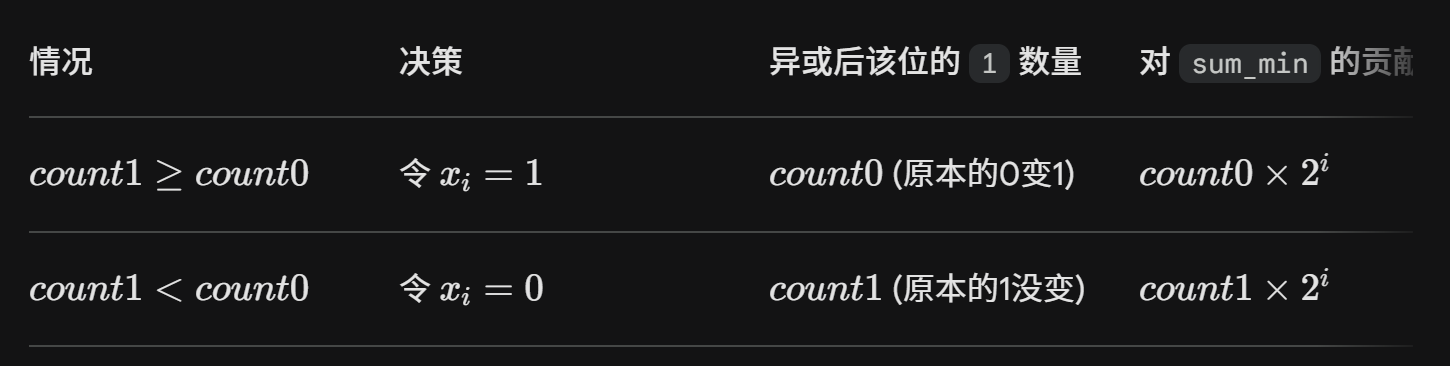
\includegraphics[width=0.8\textwidth]{figure/图示解释.png} 
	%\caption{\textbf{插图测试}}
	%\label{fig:logo}
\end{figure}
\subsubsection{P1062数列}
\item 题目链接:\href{https://www.luogu.com.cn/problem/P1062}{P1062数列(点击此处)};新颖之处:二进制求解;因为题目是选若干个k的幂的组合，所以可以用二进制的0和1做开关(每个幂都有选或不选两种选择就像二进制的0和1一样)所以\textcolor{red}{\textbf{第N项=用N的第二进制当做选幂的开关}}

代码示例:\\
\begin{lstlisting}[language=C++]
void solve() {
	ull k, n;
	cin >> k >> n;
	ull ans = 0, power = 1;
	while (n > 0) {
		if (n & 1) {  //看n的二进制最后一位是否是1，是就加幂；
			ans += power;
		}
		power *= k;
		n >>= 1; //右移更新最后一位二进制,丢掉原来的最后一位
	}
	cout << ans << endl;
}
\end{lstlisting}
\subsection{快速幂}
\subsubsection{2026天梯赛选拔1-7}
\item 题目链接：\href{https://pintia.cn/problem-sets/2030339464381566976/exam/problems/type/7?problemSetProblemId=2030339464444481542}{1-7le的7777777(点击此处)}；

\textcolor{red}{数学原理：}一个由 $n$ 个 $7$ 组成的数字可以写成如下等比数列求和的形式：$$777\dots7 (n\text{个}) = 7 \times (1 + 10^1 + 10^2 + \dots + 10^{n-1})$$利用等比数列求和公式 $S_n = \frac{a_1(q^n - 1)}{q - 1}$，其中首项 $a_1 = 1$，公比 $q = 10$：$$111\dots1 (n\text{个}) = \frac{10^n - 1}{10 - 1} = \frac{10^n - 1}{9}$$所以，最终需要计算的表达式为：$$\text{aares} = \left( 7 \times \frac{10^n - 1}{9} \right) \pmod{10^9 + 7}$$

由此数学原理的出来的最终公式可看出要使用快速幂求次方以及要利用费马小定理解题；

代码示例：\\
\begin{lstlisting}[language=C++]
ll qpow(ll a, ll b) {
	ll ans = 1;
	a %= MOD;
	while (b > 0) {
		if (b & 1)ans = (ans * a) % MOD;
		a = (a * a) % MOD;
		b >>= 1;
	}
	return ans;
}

ll feim(ll a) {
	return qpow(a, MOD - 2);
}

auto solve() -> void {
	ll n;
	cin >> n;
	ll fz = qpow(10, n);
	fz = (fz - 1 + MOD) % MOD;
	ll fm = feim(9);
	ll ans = (7 * fz) % MOD;
	ll cnt = (ans * fm) % MOD;
	cout << cnt << endl;
}
\end{lstlisting}
\subsection{单调栈}
\subsubsection{P5788单调栈模板}
\item 题目链接：\href{https://www.luogu.com.cn/problem/P5788}{P5788单调栈(点击此处)}；

代码示例：\\
\begin{lstlisting}[language=C++]
auto solve() -> void {
	ll n;
	if (!(cin >> n))return;
	vector<ll> v(n + 1), res(n + 1, 0);
	for (ll i = 1; i <= n; i++) {
		cin >> v[i];
	}
	stack<ll> st;
	for (ll i = 1; i <= n; i++) {
		while (!st.empty() && v[i] > v[st.top()]) {
			res[st.top()] = i;
			st.pop();
		}
		st.emplace(i);
	}
	for (ll i = 1; i <= n; i++) {
		cout << res[i] << " ";
	}
}
\end{lstlisting}
\subsubsection{P1318积水面积}
\item 题目链接：\href{https://www.luogu.com.cn/problem/P1318}{P1318积水面积(点击此处)}；
\textcolor{red}{注：}这题在双指针那里也有讲解，双指针是纵向相加，而单调栈是横向相加。

代码示例：\\
\begin{lstlisting}[language=C++]
class Solution {
	public:
	int trap(vector<int>& h) {
		int n = h.size();
		stack<int> s;
		int ans = 0;
		for (int i = 0; i < n; i++) {
			while (!s.empty() && h[i] > h[s.top()]) {
				int di = s.top();
				s.pop();
				if(s.empty())break;
				int left = s.top();
	//s.pop()这一步非常致命，千万不要把左边删掉了，只是借用来求最小高度，不是踢出栈外
				int w=i-left-1;
				ans += (min(h[left], h[i]) - h[di])*w;
			}
			s.emplace(i);
		}
		return ans;
	}
};
\end{lstlisting}
\subsection{其他(Luogu题库)}
\subsubsection{P3741凑VK}
\item 题目链接：\href{https://www.luogu.com.cn/problem/P3741}{P3741凑VK(点击此处)}；方法见Codeforces266B;
	
代码示例：\\
\begin{lstlisting}[language=C++]
void solve() {
	ll n, count = 0;
	string s;
	cin >> n >> s;
	for (ll i = 0; i < n - 1; i++) {
		if (s[i] == 'V' && s[i + 1] == 'K') {//只有有两个相同的就可以凑出一个VK
			count++;
			s[i]='X';
			s[i+1]='X';
		}
	}
	for (ll i=0;i<n-1;i++) {
		if (s[i]==s[i+1]&&s[i]!='X') {
			cout<<count+1<<endl;
			return;
		}
	}
	cout<<count<<endl;
}
\end{lstlisting}
\subsubsection{B3627立方根(\textcolor{red}{cbrt()函数})}
\item 题目链接：\href{https://www.luogu.com.cn/problem/B3627}{B3627立方根(点击此处)}；用库函数cbrt();

代码示例：\\
\begin{lstlisting}[language=C++]
#include <bits/stdc++.h>
using namespace std;
int main() {
	long long n,x;
	cin>>n;
	x=(long long)(cbrt(n)+1e-9);//防止形如9.999999的数字被误判为9
	//不是为了四舍五入，而是为了确保接近整数但略小时能被正确取整；
	cout<<x<<endl;
	return 0;
}
\end{lstlisting}
\subsubsection{P1765手机键盘}
\item 题目链接：\href{https://www.luogu.com.cn/problem/P1765}{P1765手机键盘(点击此处)}；总结：一定要学会\textcolor{red}{打表}，像这题还有类似剪刀石头布的那种题，打表最方便；

代码示例：\\
\begin{lstlisting}[language=C++]
int main() {
	ios_base::sync_with_stdio(false);
	cin.tie(nullptr);
	int a[26] = {1, 2, 3, 1, 2, 3, 1, 2, 3, 1, 2, 3, 1, 2, 3, 1, 2, 3, 4, 1, 2, 3, 1, 2, 3, 4};
	string s;
	int count = 0;
	getline(cin, s);
	for (int i = 0; i < s.size(); i++) {
		if (s[i] >= 'a' && s[i] <= 'z') {
			count += a[s[i] - 'a'];
		} else {
			count++;
		}
	}
	cout << count << endl;
	return 0;
}
\end{lstlisting}
\subsubsection{P5734字符串的连接,插入,截取和查找}
\item 题目链接：\href{https://www.luogu.com.cn/problem/P5734}{P5734文件处理软件(点击此处)}\textcolor{red}{模板题熟悉字符串}；

代码示例：\\
\begin{lstlisting}[language=C++]
int main() {
	int t, n;
	string s;
	cin >> t >> s;
	while (t--) {
		cin >> n;
		if (n == 1) {
			string s1;
			cin >> s1;
			s += s1;
			cout << s << endl;
		}
		if (n == 2) {
			int a, b;
			cin >> a >> b;
			s = s.substr(a, b);
			cout << s << endl;
		}
		if (n == 3) {
			int a;
			string s2;
			cin >> a >> s2;
			s.insert(a, s2);
			cout << s << endl;
		}
		if (n == 4) {
			string s3;
			cin >> s3;
			int pos = s.find(s3);
			cout << (pos != string::npos ? pos : -1) << endl;
		}
	}
	return 0;
}
\end{lstlisting}
\subsubsection{P1957区分输入个数以及保存上次输入}
\item 题目链接：\href{https://www.luogu.com.cn/problem/P1957}{P1957口算练习题(点击此处)}；总结：可以用字符串流和数组来区分输入个数，用bool类型来保存上一次输入；

代码示例：\\
\begin{lstlisting}[language=C++]
int main() {
	int i;
	cin >> i;
	char opr = '+';
	cin.ignore();
	while (i--) {
		string s;
		getline(cin, s);
		stringstream ss(s); //按空格分割字符串并存入数组
		vector<string> v;
		while (ss >> s) {
			v.push_back(s); //若输入三个则v[0]是字符，若输入2个则v[0]是数字
		}
		bool flag = false;
		if (v[0] == "a") {
			opr = '+';
			flag = true; //true则更新符号，false则保留上一次符号
		} else if (v[0] == "b") {
			opr = '-';
			flag = true;
		} else if (v[0] == "c") {
			opr = '*';
			flag = true;
		}
		string ans;
		if (flag) {  //说明v[0]是符号
			ans = v[1] + opr + v[2] + "=";
			if (opr == '+') {
				ans += to_string(atoi(v[1].c_str()) + atoi(v[2].c_str()));
			} else if (opr == '-') {
				ans += to_string(atoi(v[1].c_str()) - atoi(v[2].c_str()));
			} else if (opr == '*') {
				ans += to_string(atoi(v[1].c_str()) * atoi(v[2].c_str()));
			}
		} else {
			ans = v[0] + opr + v[1] + "=";
			if (opr == '+') {
				ans += to_string(atoi(v[0].c_str()) + atoi(v[1].c_str()));
			} else if (opr == '-') {
				ans += to_string(atoi(v[0].c_str()) - atoi(v[1].c_str()));
			} else if (opr == '*') {
				ans += to_string(atoi(v[0].c_str()) * atoi(v[1].c_str()));
			}
		}
		cout << ans << endl;
		cout << ans.size() << endl;
	}
}
\end{lstlisting}
\subsubsection{P1614队列实现循环}
\item 题目链接：\href{https://www.luogu.com.cn/problem/P1614}{P1614爱与愁的心痛(点击此处)}；

代码示例：\\
\begin{lstlisting}[language=C++]
int main() {
	i32 n,m,t,sum=0;
	cin>>n>>m;
	queue<i32> q;
	i32 min=INT_MAX;
	for (int i=0;i<n;i++) {
		cin>>t;
		q.push(t);
		if (q.size()==m) {
			sum=0;
			for (int j=0;j<m;j++) {
				sum+=q.front();
				q.push(q.front());//将每次用过的头放到对尾，保证了最后队列的顺序不变；
				q.pop();
			}
			if (sum<min) {
				min=sum;
			}
			q.pop();//删除第一组的第一个元素实现向后推进
		}
	}
	cout<<min<<endl;
	return 0;
}
\end{lstlisting}
此题也可用前缀和实现：

代码示例：\\
\begin{lstlisting}[language=C++]
int main() {
	i32 n, m;
	cin >> n >> m;
	vector<i32> v(n + 1);
	for (i32 i = 1; i <= n; i++) {
		cin >> v[i];
	}
	vector<i32> s(n + 1);
	s[0] = 0;
	for (i32 i = 1; i <= n; i++) {
		s[i] = s[i - 1] + v[i];
	}
	i32 min = INT_MAX;
	for (int i = 1; i <= n - m + 1; i++) {
		if (s[i + m - 1] - s[i - 1] < min) {
			min = s[i + m - 1] - s[i - 1];
		}
	}
	cout << min << endl;
	return 0;
}
\end{lstlisting}
\subsubsection{P1161开关和向下取整问题}
\item 题目链接：\href{https://www.luogu.com.cn/problem/P1161}{P1161开灯(点击此处)}

代码示例：\\
\begin{lstlisting}[language=C++]
#include <bits/stdc++.h>
using namespace std;
using i32 = long long;
#define N 2000005
i32 a[N];

int main() {
	ios::sync_with_stdio(false);
	cin.tie(nullptr);
	i32 n;
	cin >> n;
	while (n--) {
		double x;
		i32 t;
		cin >> x >> t;
		for (i32 i = 1; i <= t; i++) {
			if (a[(int) (x * i)] == 0) {
				a[(int) (x * i)] = 1;
			} else {
				a[(int) (x * i)] = 0;
			}
		}
	}
	for (i32 i = 0; i < N; i++) {
		if (a[i]) {
			cout << i << endl;
		}
	}
	return 0;
}
\end{lstlisting}
\subsubsection{\textcolor{red}{负数}的进制转换}
\item 题目链接：\href{https://www.luogu.com.cn/problem/P1017}{P1017进制转换(点击此处)}；

代码示例：\\
\begin{lstlisting}[language=C++]
string tobase(ll n, ll R) {
	if (n == 0)return "0";
	vector<ll> digits;
	while (n) {
		ll r = n % R;
		if (r < 0) { //当n或者R是负数的时候，余数r可能会被计算为负数
			r += abs(R);//其实就是被除数=除数*商+余数的过程
			//n+=1        //这样写也可以，在纸上算一下就知道了
			n = (n - r) / R;//因为R变成正数所以商也要做出改变
		} else {
			n /= R;
		}
		digits.push_back(r);
	}
	string rem;
	for (ll i = digits.size() - 1; i >= 0; i--) {
		ll d = digits[i];
		if (d < 10)rem += to_string(d);
		else rem += 'A' + d - 10;
	}
	return rem;
}
void solve() {
	ll n, R;
	cin >> n >> R;
	string s;
	s = tobase(n, R);
	cout << to_string(n) << "=" << s << "(base" << R << ")" << endl;
}
\end{lstlisting}
\subsubsection{P1061循环递增字母序列}
\item 题目链接：\href{https://www.luogu.com.cn/problem/P1061}{p1061Jam的计数法(点击此处)}；

代码示例：\\
\begin{lstlisting}[language=C++]
void solve(){
	ll s,t,w;
	string st;
	cin>>s>>t>>w>>st;
	for(ll i=1;i<=5;++i){
		for(ll j=w-1;j>=1;--j){
			if(st[j]-'a'+1<=t-(w-j)){//防止最后几位加1时越界
				st[j]++;
				for(ll k=j+1;k<w;++k){
					st[k]=st[k-1]+1;
				}
				cout<<st<<endl;
				break;
			}
		}
	}
}
\end{lstlisting}
\subsubsection{字串成比例数字查找}
\item 题目链接：\href{https://www.luogu.com.cn/problem/P1008}{P1008三连击(点击此处)}；总结：这是技巧性的东西，可以积累一下。

代码示例：\\
\begin{lstlisting}[language=C++]
bool ok(ll a, ll b, ll c) {
	string s = to_string(a) + to_string(b) + to_string(c);
	if (s.size() != 9)return false;
	sort(s.begin(), s.end());
	return s == "123456789";
}

void solve() {
	ll a, b, c;
	for (a = 160; a <= 360; ++a) {//这个范围可通过暴力打表找出
		b = a * 2;
		c = a * 3;
		if (ok(a, b, c)) {
			cout << a << " " << b << " " << c << endl;
		}
	}
}
\end{lstlisting}
暴力打表：对这题而言即用全排列列出所有可能然后输出满足条件的数
\subsubsection{解二元一次方程组(sscanf的用法)}
\item \textcolor{red}{解释：此题为偶然间发现的题并非来自做题网站但是题目很直接。}
\section*{C++ 中的 sscanf 深度解析}

\subsection*{1. 核心定义与引入}
在 C++ 中，推荐包含 \texttt{<cstdio>} 而非 \texttt{<stdio.h>}。虽然 \texttt{sscanf} 是 C 风格的函数，但在处理格式化字符串解析时，其性能通常优于 \texttt{stringstream}。

\[ \text{int sscanf(const char *buffer, const char *format, ...);} \]

\begin{quote}
	\textbf{注意：} \texttt{sscanf} 只能直接操作 \texttt{const char*}。如果你使用的是 \texttt{std::string}，必须调用 \texttt{.c\_str()} 方法。
\end{quote}

\subsection*{2. 格式化匹配高级技巧}
\texttt{sscanf} 的强大之处在于其格式控制符的组合能力：

\begin{itemize}
	\item \textbf{忽略特定项 (\%*)}: 
	使用 \texttt{\%*d} 或 \texttt{\%*s} 可以跳过不需要的数据，不进行赋值。
	\item \textbf{字符集匹配 (\%[ ])}:
	\begin{itemize}
		\item \texttt{\%[a-z]}: 匹配任意小写字母。
		\item \texttt{\%[\^{}\textbackslash n]}: 读取直到换行符为止（常用于读取带空格的整行）。
	\end{itemize}
	\item \textbf{宽度限制}: \texttt{\%10s} 限制最多读取 10 个字符，防止缓冲区溢出。
\end{itemize}

\subsection*{3. 典型应用场景示例}

\begin{table}[h]
	\centering
	\begin{tabular}{|l|l|l|}
		\hline
		\textbf{任务} & \textbf{格式字符串} & \textbf{说明} \\ \hline
		解析 IP 地址 & \texttt{"\%d.\%d.\%d.\%d"} & 将点分十进制解析为 4 个整数 \\ \hline
		提取括号内容 & \texttt{"\%*[\^{}(](\%[\^{}])"} & 跳过左括号前的内容，提取括号内内容 \\ \hline
		过滤非数字 & \texttt{"\%*[\^{}0-9]\%d"} & 跳过前导非数字字符，读取第一个数字 \\ \hline
	\end{tabular}
\end{table}

\subsection*{4. C++ 实践代码片段}
\begin{verbatim}
	#include <cstdio>
	#include <string>
	#include <vector>
	
	void demo() {
		std::string data = "ID:1024, Score:98.5, Name:Alice";
		int id;
		float score;
		char name[20];
		
		// C++ 中必须使用 .c_str()
		int count = sscanf(data.c_str(), "ID:%d, Score:%f, Name:%s", &id, &score, name);
		
		if (count == 3) {
			// 成功解析所有字段
		}
	}
\end{verbatim}

\subsection*{5. sscanf vs std::stringstream}
\begin{itemize}
	\item \textbf{性能}: \texttt{sscanf} 通常比 \texttt{std::stringstream} 快 3-10 倍。
	\item \textbf{安全性}: \texttt{stringstream} 更安全，会自动处理内存；\texttt{sscanf} 需要预先分配 \texttt{char} 数组，存在溢出风险。
	\item \textbf{灵活性}: \texttt{sscanf} 的模式匹配（如 \texttt{\%[\^{},]}）在处理复杂分隔符时比 \texttt{getline} 更简洁。
\end{itemize}

\subsection*{6. 常见陷阱 (Pitfalls)}
\begin{enumerate}
	\item \textbf{指针传递}: 必须传递变量地址（\texttt{\&var}），否则会导致段错误（Segmentation Fault）。
	\item \textbf{数组越界}: 解析字符串到 \texttt{char[]} 时，务必指定最大宽度，如 \texttt{\%19s} 对应 \texttt{char[20]}。
	\item \textbf{返回值检查}: 始终检查返回值是否等于预期的参数个数，以确保数据的完整性。
\end{enumerate}
代码示例：\\
\begin{lstlisting}[language=C++]
class System {
	private:
	double a = 0, b = 0, c = 0, d = 0, e = 0, f = 0;
	
	public:
	auto input() -> void {
		string s;
		getline(cin, s);
		ll count = sscanf(s.c_str(), "%lfx+%lfy=%lf;%lfx+%lfy=%lf", &a, &b, &c, &d, &e, &f);
		if (count < 6) {
			cout << "警告：输入格式解析不完整，请确保包含所有系数和符号！" << endl;
		}
	}
	
	auto solve() -> void {
		double D = a * e - b * d;
		if (D != 0) {
			const double x = (c * e - b * f) / D;
			const double y = (a * f - c * d) / D;
			printf("方程组的解为：x = %.2f, y = %.2f\n", x, y);
		} else {
			if ((a * f - c * d) == 0 && (c * e - b * f) == 0) {
				cout << "方程组有无数个解。" << endl;
			} else {
				cout << "方程组无解。" << endl;
			}
		}
	}
};

int main() {
	ios::sync_with_stdio(false);
	cin.tie(nullptr);
	System sys;
	sys.input();
	sys.solve();
	return 0;
}
\end{lstlisting}
\subsubsection{P5250 set的用法}
\item 题目链接:\href{https://www.luogu.com.cn/problem/P5250}{P5250木材仓库(点击此处)}；\textcolor{red}{STL的用法必须积累和记忆，非常重要！}

代码示例：\\
\begin{lstlisting}[language=C++]
auto solve() -> void {
	ll n;
	cin >> n;
	set<ll> st;
	while (n--) {
		ll q, l;
		cin >> q >> l;
		if (q == 1) {
			if (st.count(l)) cout << "Already Exist" << endl;
			else st.insert(l);
		} else {
			if (st.empty()) {
				cout << "Empty" << endl;
			} else {
			//lower_bound函数是用在数组vector里面的，但是在set中是它自配的函数表示
			//第一个>=l的数的下标。
			//在vector中为id=lower_bound(v.begin(),v.end(),x)-v.begin();
				auto it = st.lower_bound(l);
				//若it==st.begin()说明所有数都大于l
				if (it == st.begin()) {
					cout << *it << endl;
					st.erase(it);
				//若it==st.end()说明所有数都小于l
				} else if (it == st.end()) {
					it--;
					cout << *it << endl;
					st.erase(it);
				} else {
				//prev(it)是指it迭代器所指元素的上一个元素，即最后一个<l的数。
					auto pre = prev(it);
					ll dist_pre = l - *pre;
					ll dist_next = *it - l;
					if (dist_pre > dist_next) {
						cout << *it << endl;
						st.erase(it);
					} else {
						cout << *pre << endl;
						st.erase(pre);
					}
				}
			}
		}
	}
}
\end{lstlisting}
\subsubsection{P1056排座位}
\item 题目链接：\href{https://www.luogu.com.cn/problem/P1056}{P1056排座位(点击此处)}；

代码示例：\\
\begin{lstlisting}[language=C++]
//用结构体是为了方便后续的排序，也可换成vector<pair<ll,ll>>.
struct med {
	ll num, p;
} row[1005], col[1005];
//使结构体在前k个横列和前l个纵列可以分开的对数最多
auto cmp1(const med &a, const med &b) -> bool {
	return a.num > b.num;
}
//为了满足序号从小到大
auto cmp2(const med &a, const med &b) -> bool {
	return a.p < b.p;
}

auto solve() -> void {
	ll m, n, k, l, d;
	cin >> m >> n >> k >> l >> d;
	for (ll i = 0; i < d; i++) {
		ll x1, y1, x2, y2;
		cin >> x1 >> y1 >> x2 >> y2;
		if (x1 == x2) {
		//col[]内部的下标是为了防止后续同样的纵列依旧新增数组大小
		//目的是吧同一个纵列或行列所能分开的对数最大化(贪心思想)
			col[min(y1, y2)].p = min(y1, y2);
			col[min(y1, y2)].num++;
		} else {
			row[min(x1, x2)].p = min(x1, x2);
			row[min(x1, x2)].num++;
		}
	}
	sort(row, row + m, cmp1);
	sort(col, col + n, cmp1);
	sort(row, row + k, cmp2);
	sort(col, col + l, cmp2);
	for (ll i = 0; i < k; i++) {
		cout << row[i].p << " ";
	}
	cout << endl;
	for (ll i = 0; i < l; i++) {
		cout << col[i].p << " ";
	}
}
\end{lstlisting}
\subsubsection{P1072最大公因数(约数)和最小公倍数}
\item 题目链接：\href{https://www.luogu.com.cn/problem/P1072}{P1072趣味数学(点击此处)}；\textcolor{purple}{x和b0的最小公倍数是b1说明x和b0都是b1的因数(约数)}；\\
\textcolor{red}{约数(因数)：}\textbf{定义：}如果整数 $a$ 除以整数 $b$ 的余数为 $0$，那么 $b$ 就是 $a$ 的约数。
\textbf{例子：}
\begin{itemize}
	\item $6$ 的约数有 $1, 2, 3, 6$。
\end{itemize}
\textcolor{red}{最大公因数：}\textbf{定义：}两个或多个整数共有约数中最大的那个，称为\textbf{最大公约数(gcd)}
\textbf{例子：}
\begin{itemize}
	\item $12$ 的约数集合为 $A = \{1, 2, 3, 4, 6, 12\}$
	\item $18$ 的约数集合为 $B = \{1, 2, 3, 6, 9, 18\}$
\end{itemize}
\textcolor{red}{最小公倍数：}\textbf{定义：}两个或多个整数公有的倍数中最小的正整数,称为\textbf{最小公倍数(lcm)};
\begin{itemize}
	\item $4$ 的倍数有 $\{4, 8, 12, 16, \dots\}$，$6$ 的倍数有 $\{6, 12, 18, \dots\}$。他们最小公共倍数是12.
	\item 数学公式：$\text{lcm}(a, b) = \frac{|a \times b|}{\gcd(a, b)}$。
\end{itemize}
代码示例：\\
\begin{lstlisting}[language=C++]
auto lcm(const ll a, const ll b) -> ll {
	return a / gcd(a, b) * b;
}

auto solve() -> void {
	ll cnt = 0;
	ll a0, a1, b0, b1;
	cin >> a0 >> a1 >> b0 >> b1;
	for (ll x = 1; x * x <= b1; x++) {
		if (b1 % x == 0) {
			if (gcd(a0, x) == a1 && lcm(x, b0) == b1) {
				cnt++;
			}
			//注意这里之前说过：若x是b1的因数，则b1/x也是b1的因数
			ll d = b1 / x;
			if (d != x) {
				if (gcd(a0, d) == a1 && lcm(d, b0) == b1) {
					cnt++;
				}
			}
		}
	}
	cout << cnt << endl;
}
\end{lstlisting}
\subsubsection{康托尔折线(z字形--蛇形矩阵遍历)}
\item 题目链接:\href{https://www.luogu.com.cn/problem/P1014}{P1014 Cantor表(点击此处)}；
\textcolor{red}{注意：}这里的蛇形遍历是指对角线的蛇形而不是行或者列的蛇形。
代码示例：\\
\begin{lstlisting}[language=C++]
auto solve() -> void {
	ll n;
	cin >> n;
	ll row = 1;
	while (n > row) {
		n -= row;
		row++;
	}
	if (row & 1) {
		cout << (row - n + 1) << "/" << n << endl;
	} else {
		cout << n << "/" << (row - n + 1) << endl;
	}
}
\end{lstlisting}
\subsubsection{异或和的特性及用法}
\item 题目链接：\href{https://www.luogu.com.cn/problem/P1469}{P1469找筷子(点击此处)}；
\textcolor{red}{注意：此题内存给的极少，但是数据范围很大，不能开map等其他容器}；

\textcolor{orange}{原理(异或的性质)：}
\section*{异或运算（XOR）的核心特性}

异或运算（在 C++ 中为 \texttt{\^}）具有以下三个对本题至关重要的特性：

\begin{enumerate}
	\item \textbf{自反性：} 任何数与自身异或结果为 0。
	\[ x \oplus x = 0 \]
	
	\item \textbf{恒等律：} 任何数与 0 异或结果保持不变。
	\[ x \oplus 0 = x \]
	
	\item \textbf{结合律与交换律：} 运算顺序不影响结果，成对的数可以抵消。
	\begin{align*}
		a \oplus b \oplus a &= (a \oplus a) \oplus b \\
		&= 0 \oplus b \\
		&= b
	\end{align*}
\end{enumerate}
代码示例：\\
\begin{lstlisting}[language=C++]
auto solve() -> void {
	ll n;
	cin >> n;
	ll ans = 0;
	for (ll i = 0; i < n; i++) {
		ll x;
		cin >> x;
		ans ^= x;
	}
	cout << ans << endl;
}
\end{lstlisting}
\end{itemize}
\newpage

































\section{lanqiao刷题总结}
%\textcolor{blue}{\textbf{271A}}
%\begin{lstlisting}[language=C++]\end{lstlisting}
%\textcolor{red}{\textbf{注意：}}
在本节中，我将总结我在 lanqiao 上做题的经验。

\subsection{遇到的问题以及学到的方法}
\begin{itemize}
\subsubsection{最少回文子串}
\item 题目链接:\href{https://www.lanqiao.cn/problems/21192/learning/?contest_id=274}{最少子串回文数(点击此处)};方法：1、\textcolor{red}{\textbf{回文数特点(非常重要！！！):}}最多允许一个字符出现奇数次(要么所有字符的出现次数都为偶数，要么只能有一个字符出现次数为奇数(\textcolor{blue}{\textbf{出现在中心位置}}));2、总结:若所有字符出现次数均为偶数则答案为1；否则答案是出现次数为奇数的字符的个数；
	
代码示例:\\
\begin{lstlisting}[language=C++]
#include <bits/stdc++.h>
using namespace std;
int main(){
	int n;
	string s;
	cin>>n>>s;
	vector<int> v(26,0);
	for(auto x:s){
		v[x-'a']++;
	}
	int odd_cnt=0;
	for(auto ch:v){
		if(ch&1){
			odd_cnt++;
		}
	}
	if(odd_cnt==0) cout<<1<<endl;
	else cout<<odd_cnt<<endl;
	return 0;
}
\end{lstlisting}
\subsubsection{合理配置}
\item 题目链接 \href{https://www.lanqiao.cn/problems/21193/learning/?contest_id=274}{合理配置(点击此处)}；思路用总的袋子数-合理配置的数量=幽默配置的数量；
	
代码示例：\\
\newpage
\begin{lstlisting}[language=C++]
#include <bits/stdc++.h>
#define endl '\n'
using namespace std;
using ll=long long;
int main(){
	ll a,b;
	cin>>a>>b;
	ll ans=INT_MAX;
	for(ll i=0;i<=min(a,b);i++){
		ans=min(ans,abs(a+b-4*i));
	}
	cout<<ans<<endl;
	return 0;
}
\end{lstlisting}
\end{itemize}






















\section{PTA 刷题总结}
%\textcolor{blue}{\textbf{271A}}
%\begin{lstlisting}[language=C++]\end{lstlisting}
在本节中，我将总结我在 PTA 上做题的经验。

\subsection{遇到的问题以及学到的方法}
\begin{itemize}
\subsection{对数组每一列按升序排序}
\item 题目链接：\href{https://pintia.cn/problem-sets/1997490617200599040/exam/problems/type/7?problemSetProblemId=1997490617559937029}{坚固矩阵(点击此处)}；						

代码示例：\\
\begin{lstlisting}[language=C++]
void solve() {
	ll n, m;
	cin >> n >> m;
	vector<vector<ll> > v(n, vector<ll>(m));
	for (ll i = 0; i < n; i++) {
		for (ll j = 0; j < m; j++) {
			cin >> v[i][j];
		}
	}
	for (ll j = 0; j < m; j++) {
		//开一个新数组来存每一列的数字，然后排序；
		vector<ll> a;
		for (ll i = 0; i < n; i++) {
			a.push_back(v[i][j]);
		}
		sort(a.begin(), a.end());
		//将排序好的数组在放进原数组中；
		for (ll i = 0; i < n; i++) {
			v[i][j] = a[i];
		}
	}
	bool flag;
	for (ll i = 0; i < n; i++) {
		flag = true;
		for (ll j = 0; j < m; j++) {
			cout << (flag == true ? "" : " ") << v[i][j];
			flag = false;
		}
		cout << endl;
	}
}
\end{lstlisting}
\subsection{轮流问题}
\item 题目链接：\href{https://pintia.cn/problem-sets/1997490617200599040/exam/problems/type/7?problemSetProblemId=1997490617559937026}{小杭玩游戏(点击此处)}；总结：可以用bool来表示轮到谁了。

代码示例：\\
\begin{lstlisting}[language=C++]
void solve() {
	ll a,b,n,cnt=0;
	cin>>a>>b>>n;
	bool flag=true;
	while(n>0){
		ll m;
		cnt++;
		if(flag){
			m=gcd(n,a);
		}else{
			m=gcd(n,b);
		}
		n-=m;
		flag=!flag;
	}
	if(flag){
		cout<<"Xiao Hong Win"<<endl;
		cout<<cnt<<endl;
	}else{
		cout<<"Xiao Ming Win"<<endl;
		cout<<cnt<<endl;
	}
}
\end{lstlisting}
\subsection{结构体的使用}
\item 题目链接：\href{https://pintia.cn/problem-sets/994805046380707840/exam/problems/type/7?problemSetProblemId=994805071789801472&page=1}{L2-003月饼(点击此处)}；\\\textcolor{red}{总结：当要记录多个数据(两个以上)时可以用结构体来操作。}处理两个数据可以用哈希表或者其他容器操作。
\\lambda函数也要了解一下。

代码示例：\\
\begin{lstlisting}[language=C++]
class total {
	public:
	double w;
	double v;
	double d;
};

bool cmp(total t1, total t2) {
	return t1.d > t2.d;
}

void solve() {
	ll n;
	double m;
	cin >> n >> m;
	vector<total> a(n);
	for (ll i = 0; i < n; i++) {
		cin >> a[i].w;
	}
	for (ll i = 0; i < n; i++) {
		cin >> a[i].v;
		a[i].d = a[i].v / a[i].w;
	}
	sort(a.begin(), a.end(), cmp);
	//也可以写成lambda函数的形式
	//  sort(a.begin(),a.end(),[](total &t1,total &t2){
		//          return t1.d>t2.d;
		//  });
	double ans = 0;
	for (ll i = 0; i < n && m > 0; i++) {
		if (a[i].w <= m) {
			ans += a[i].v;
			m -= a[i].w;
		} else {
			ans += a[i].d * m;
			m = 0;
		}
	}
	cout << fixed << setprecision(2) << ans << endl;
}
\end{lstlisting}
\subsection{固定位数问题}
\item 题目链接：\href{https://pintia.cn/problem-sets/994805046380707840/exam/problems/type/7?problemSetProblemId=994805099426070528}{出生年(点击此处)}  总结：set去重可以检查有几个不同，for循环固定4次，就算temp=0也要继续循环，保证了始终有四位。

代码示例：\\
\begin{lstlisting}[language=C++]
int main() {
	int y, n;
	cin >> y >> n;
	for (int i = y; ; i++) {
		set<int> st;
		int temp = i;
		for (int j = 0; j < 4; j++) {
			st.insert(temp % 10);
			temp /= 10;
		}
		if (st.size() == n) {
			printf("%d %04d", i - y, i);
			return 0;
		}
	}
}
\end{lstlisting}
\subsubsection{字符串查找连续满足条件串的方法}
\item 题目链接：\href{https://pintia.cn/problem-sets/994805046380707840/exam/problems/type/7?problemSetProblemId=1111914599408664577}{L1-058 6翻了(点击此处)}；

代码示例：\\
\begin{lstlisting}[language=C++]
auto solve() -> void {
	string s;
	getline(cin, s);
	for (ll i = 0; i < s.size();) {
		if (s[i] == '6') {
			ll cnt = 0;
			ll j = i;
			//改成while循环代替之前的cnt=0和！=0的分类讨论
			//尽量用这种思想替换掉以取的思想
			while (j < s.size() && s[j] == '6') {
				cnt++;
				j++;
			}
			if (cnt > 9) {
				cout << "27";
			} else if (cnt > 3) {
				cout << "9";
			} else {
				for (ll k = 0; k < cnt; k++) {
					cout << "6";
				}
			}
			i = j;
		} else {
			cout << s[i];
			i++;
		}
	}
}
\end{lstlisting}
\subsubsection{活用字符串字串提取函数(substr)}
\item 题目链接：\href{https://pintia.cn/problem-sets/994805046380707840/exam/problems/type/7?problemSetProblemId=1111914599412858880}{L1-059 敲笨钟(点击此处)}；

代码示例：\\
\begin{lstlisting}[language=C++]
auto solve() -> void {
	string s;
	getline(cin, s);
	//要熟练的使用find和substr函数，对字符串的提取和替换都有很大的作用
	size_t pos1 = s.find(',');
	size_t pos2 = s.find('.');
	bool flag = false;
	if (pos1 >= 3 && pos2 >= 3) {
		if (s.substr(pos1 - 3, 3) == "ong" && s.substr(pos2 - 3, 3) == "ong") {
			flag = true;
		}
	}
	if (!flag) {
		cout << "Skipped" << endl;
	} else {
		ll i = s.size() - 1;
		ll cnt = 0;
		while (i > 0) {
			if (s[i] == ' ') {
				cnt++;
			}
			if (cnt == 3) {
				break;
			}
			i--;
		}
		//这种输出之前也没有见过，要学习一下，不要再一个一个遍历s再存t了
		cout << s.substr(0, i + 1) << "qiao ben zhong." << endl;
	}
}
\end{lstlisting}
\subsubsection{最小化思想2026天梯选拔赛1-6}
\item 题目链接：\href{https://pintia.cn/problem-sets/2030339464381566976/exam/problems/type/7?problemSetProblemId=2030339464444481541}{1-6源初之石(点击此处)}；

代码示例：\\
\begin{lstlisting}[language=C++]
auto solve() -> void {
	ll n;
	cin >> n;
	ll a = -1, b = -1, c = -1;
	//之所以要看i*i*i是为了找到能使三个数相乘=n的最小值(这里默认把最小值给了a)；
	for (ll i = 2; i * i * i <= n; i++) {
		if (n % i == 0) {
			a = i;
			break;
		}
	}
	if (a == -1) {
		cout << "NO" << endl;
		return;
	}
	//因为前面的a已经使最小的了所以这里找c的时候可以从a+1开始找，可以提高效率。
	for (ll i = a + 1; i * i <= n / a; i++) {
		if ((n / a) % i == 0) {
			c = i;
			b = n / a / c;
			if (b >= 2 && b != a && b != c) {
				cout << "YES" << endl;
				cout << a << " " << c << " " << b << endl;
				return;
			}
		}
	}
	cout << "NO" << endl;
}
\end{lstlisting}
\end{itemize}
\newpage



























\section{AtCoder刷题总结}
%\textcolor{blue}{\textbf{271A}}
%\begin{lstlisting}[language=C++]\end{lstlisting}
%\textcolor{red}{\textbf{注意：}}
在本节中，我将总结我在 AtCoder 上做题的经验。

\subsection{遇到的问题以及学到的方法}
\begin{itemize}
\subsection{}
\item 题目链接：\href{}{}
代码示例：\\
\begin{lstlisting}[language=C++]

\end{lstlisting}
\end{itemize}
\newpage
\section{AcWing刷题总结}
%\textcolor{blue}{\textbf{271A}}
%\begin{lstlisting}[language=C++]\end{lstlisting}
%\textcolor{red}{\textbf{注意：}}
在本节中，我将总结我在 AcWing 上做题的经验。

\subsection{遇到的问题以及学到的方法}
\begin{itemize}
\subsection{2816判断子序列}
\item 题目链接：\href{https://www.acwing.com/problem/content/2818/}{2816判断子序列(点击此处)}；
代码示例：\\
\begin{lstlisting}[language=C++]
auto solve() -> void {
	ll n, m;
	cin >> n >> m;
	queue<ll> q1, q2;
	for (ll i = 0; i < n; i++) {
		ll a;
		cin >> a;
		q1.emplace(a);
	}
	for (ll i = 0; i < m; i++) {
		ll b;
		cin >> b;
		q2.emplace(b);
	}
	while (q1.size() && q2.size()) {
		if (q1.front() == q2.front()) {
			q1.pop();
			q2.pop();
		} else {
			q2.pop();
		}
	}
	if (q1.size() == 0) {
		cout << "Yes" << endl;
	} else if (q2.size()==0){
		cout << "No" << endl;
	}
}
\end{lstlisting}
\end{itemize}
\newpage

%\section{demo}

测试文字

%
%摘要部分
\begin{abstract}
	这是摘要的第一段这是摘要的第一段这是摘要的第一段这是摘要的第一段这是摘要的第一段这是摘要的第一段这是摘要的第一段这是摘要的第一段这是摘要的第一段这是摘要的第一段这是摘要的第一段这是摘要的第一段这是摘要的第一段这是摘要的第一段这是摘要的第一段这是摘要的第一段这是摘要的第一段这是摘要的第一段这是摘要的第一段这是摘要的第一段这是摘要的第一段这是摘要的第一段这是摘要的第一段这是摘要的第一段这是摘要的第一段这是摘要的第一段这是摘要的第一段这是摘要的第一段这是摘要的第一段这是摘要的第一段这是摘要的第一段这是摘要的第一段这是摘要的第一段这是摘要的第一段这是摘要的第一段这是摘要的第一段
	
	这是摘要的第二段这是摘要的第二段这是摘要的第二段这是摘要的第二段这是摘要的第二段这是摘要的第二段这是摘要的第二段这是摘要的第二段这是摘要的第二段这是摘要的第二段这是摘要的第二段这是摘要的第二段这是摘要的第二段这是摘要的第二段这是摘要的第二段这是摘要的第二段这是摘要的第二段这是摘要的第二段这是摘要的第二段这是摘要的第二段这是摘要的第二段这是摘要的第二段这是摘要的第二段这是摘要的第二段这是摘要的第二段这是摘要的第二段这是摘要的第二段这是摘要的第二段这是摘要的第二段这是摘要的第二段这是摘要的第二段这是摘要的第二段这是摘要的第二段这是摘要的第二段这是摘要的第二段这是摘要的第二段这是摘要的第二段这是摘要的第二段这是摘要的第二段这是摘要的第二段这是摘要的第二段这是摘要的第二段这是摘要的第二段这是摘要的第二段这是摘要的第二段这是摘要的第二段
	
	
	超链接:
	
	\url{https://baidu.com}
	
	\href{https://bing.com}{必应官网}
	
	\textbf{\color{blue}关键字:\quad 关键字1 \quad 关键字2 \quad 关键字3}
	
\end{abstract}


\newpage

\section{这是第一章的一级标题}
\subsection{这是第一章的二级标题}
\subsubsection{这是第一章的三级标题}

\newpage

\section{图片示例}
\subsection{单张图片插入示例}
\begin{figure}[H]
	\centering
	
\includegraphics[width=0.5\textwidth]{figure/xcpclogo.png} 
	\caption{\textbf{这是图片标题}}
	\label{fig:test1}
\end{figure}

这是图片\ref{fig:test1}

\subsection{多张图片插入示例}

\begin{figure}[H]
	\centering
	\begin{minipage}[c]{0.3\textwidth}
		\centering
		
\includegraphics[width=0.95\textwidth]{figure/xcpclogo.png} 
		\label{fig:sample-figure-a}
	\end{minipage}
	\begin{minipage}[c]{0.3\textwidth}
		\centering
		
\includegraphics[width=0.95\textwidth]{figure/xcpclogo.png} 
		\label{fig:sample-figure-b}
	\end{minipage}
	\begin{minipage}[c]{0.3\textwidth}
		\centering
		
\includegraphics[width=0.95\textwidth]{figure/xcpclogo.png} 
		\label{fig:sample-figure-c}
	\end{minipage}
	\caption{多图并排示例}
	\label{fig:sample-figure}
\end{figure}

\newpage

\section{表格相关}

\begin{table}[H]
	\caption{标准三线表格}
	\label{tab:001} 
	\centering
	\begin{tabular}{cccccc}
		\toprule[1.5pt]
		$D$(in) & $P_u$(lbs) & $u_u$(in) & $\beta$ & $G_f$(psi.in) & $G_f$(psi.in) \\
		\midrule[1pt]
		5 & 269.8 & 0.000674 & 1.79 & 0.04089 & 0.04089\\
		10 & 421.0 & 0.001035 & 3.59 & 0.04089 & 0.04089 \\
		20 & 640.2 & 0.001565 & 7.18 & 0.04089 & 0.04089\\
		20 & 640.2 & 0.001565 & 7.18 & 0.04089 & 0.04089\\
		20 & 640.2 & 0.001565 & 7.18 & 0.04089 & 0.04089\\
		20 & 640.2 & 0.001565 & 7.18 & 0.04089 & 0.04089\\
		20 & 640.2 & 0.001565 & 7.18 & 0.04089 & 0.04089\\
		20 & 640.2 & 0.001565 & 7.18 & 0.04089 & 0.04089\\
		\bottomrule[1.5pt]
	\end{tabular}
\end{table}

\newpage

\section{公式}

首先是行内公式，例如 $ \theta $ 是角度。行内公式使用 \verb|$  $| 包裹。

行间公式不需要编号的可以使用 \verb|\[  \]| 包裹，例如
\[
E_1=mc^2
\]
其中 $ E $ 是能量，$ m $ 是质量，$ c $ 是光速。

如果希望某个公式带编号，并且在后文中引用可以参考下面的写法：
\begin{equation}
	E=mc^2
	\label{eq:energy}
\end{equation}
式\ref{eq:energy}是质能方程。


多行公式有时候希望能够在特定的位置对齐，以下是其中一种处理方法。
\begin{align}
	P & = UI \\
	& = I^2R
\end{align}
\verb|&| 是对齐的位置， \verb|&| 可以有多个，但是每行的个数要相同。

矩阵的输入也不难。
\[
\mathbf{X} = \left(
\begin{array}{cccc}
	x_{11} & x_{12} & \ldots & x_{1n}\\
	x_{21} & x_{22} & \ldots & x_{2n}\\
	\vdots & \vdots & \ddots & \vdots\\
	x_{n1} & x_{n2} & \ldots & x_{nn}\\
\end{array} \right)
\]

分段函数这些可以用 \verb|case| 环境，但是它要放在数学环境里面。
\[
f(x) =
\begin{cases}
	0 &  x \text{为无理数} ,\\
	1 &  x \text{为有理数} .
\end{cases}
\]

在数学环境里面，字体用的是数学字体，一般与正文字体不同。假如要公式里面有个别文字，则需要把这部分放在 \verb|text| 环境里面，即 \verb|\text{文本环境}| 。比如$3x+5a+\text{文字}+999$

\newpage

\section{杂项}

\subsection{脚注}

利用 \verb|\footnote{具体内容}| 可以生成脚注\footnote{脚注可以补充说明一些东西}。

\subsection{无序列表与有序列表}

无序列表是这样的：
\begin{itemize}
	\item one
	\item two
	\item three
\end{itemize}

有序列表是这样子的：
\begin{enumerate}
	\item[(1)] 1111
	\item[(2)] 2222
	\item[(3)] 3333
\end{enumerate}


1.请做出正确选项(\quad )
\begin{choices}
	\item 选项2选项
	\item 选项2选项1
	\item 选项3选项1选项1
	\item 选项4选项1
\end{choices}

\subsection{字体加粗与斜体}

如果想强调部分内容，可以使用加粗的手段来实现。加粗字体可以用 \verb|\textbf{加粗}| 来实现。例如： \textbf{这是加粗的字体。 This is bold fonts} 。

中文字体没有斜体设计，但是\cite{testcite3}英文字体有。\textit{斜体 Italics}。

\newpage

\section{代码}

\begin{lstlisting}[language=sql,caption={MySql代码}]
-- 显示数据库
show databases;
-- 创建数据库
create database if not exists game;
-- 创建表
create table if not exists player
(
id    int primary key not null auto_increment,
name  varchar(100),
level int,
exp   int,
gold  decimal(10, 2)
);
-- 查看表结构
desc player;
-- 修改行关键字的数据类型
alter table player
modify column name varchar(200);
-- 修改行关键字的名称
alter table player
rename column name to nickname;
\end{lstlisting}

\begin{lstlisting}[language=c++,caption={C++代码测试}]
#include<bits/stdc++.h>
using namespace std;
struct Student {
	string name;
	int score;
};

bool cmp(const Student& a, const Student& b) {
	if (a.score != b.score) {
		return a.score > b.score;
	} else {
		return a.name < b.name;
	}
}

int main()
{
	int n;
	cin >> n;
	vector<Student> students(n);
	for (int i = 0; i < n; ++i) {
		cin >> students[i].name >> students[i].score;
	}
	sort(students.begin(), students.end(), cmp);
	for (const auto& student : students) {
		cout << student.name << "," << student.score << endl;
	}
	return 0;
}
\end{lstlisting}


\newpage

\section{参考文献与引用}

参考文献对于一篇正式的论文来说是必不可少的，论文中重要的参考文献当然应该列出。\LaTeX{}在这方面的功能也是十分强大的，下面进介绍一个比较简单的参考文献制作方法。有兴趣的可以学习 \verb|bibtex| 或 \verb|biblatex| 的使用。

这是一个引用\cite{testcite1}。这是一个简单的引用，用 \verb|\cite{bibkey}| 来完成。要引用成功，当然要维护好 bibitem 了。下面是个简单的例子。



%参考文献
\begin{thebibliography}{9}%宽度9
	\bibitem[1]{testcite1}
	姜振坤
	\newblock 河北工程大学,
	\newblock 信息与电气工程学院.
	
	\bibitem[2]{testcite2}
	张三
	\newblock 河北工程大学,
	\newblock 信息与电气工程学院.
	
	\bibitem[3]{testcite3}
	李四
	\newblock 河北工程大学,
	\newblock 信息与电气工程学院.
	
	\bibitem[4]{testcite4}
	王五
	\newblock 河北工程大学,
	\newblock 信息与电气工程学院.
	
	\bibitem[5]{testcite5}
	赵六
	\newblock 河北工程大学,
	\newblock 信息与电气工程学院.
	
\end{thebibliography}






%%基础算法
%\section{基础算法}




%\subsection{高精度计算}


\subsection{二分查找算法}

\begin{lstlisting}[language=c++,caption={查找最后一个小于等于q的数的下标}]
//查找最后一个小于等于q的数的下标
int find(int q) {
	int l = 0, r = n + 1; //开区间
	while (l + 1 < r) {
		// l + 1 < r时结束
		int mid = l + r >> 1;
		if (a[mid] <= q) {
			l = mid;
		} else {
			r = mid;
		}
	}
	return l;
}
\end{lstlisting}

\begin{lstlisting}[language=c++,caption={查找第一个大于等于q的数的下标}]
//查找第一个大于等于q的数的下标
int find(int q) {
	int l = 0, r = n + 1; //开区间
	while (l + 1 < r) {
		// l + 1 < r时结束
		int mid = l + r >> 1;
		if (a[mid] >= q) {
			r = mid;
		} else {
			l = mid;
		}
	}
	return r;
}

\end{lstlisting}

\begin{lstlisting}[language=c++,caption={洛谷P2249 查找}]
//洛谷P2249 【深基13.例1】查找
//询问数字,输出这个数字在序列中第一次出现的编号，如果没有找到的话输出 −1 
#include<bits/stdc++.h>
using namespace std;
int main() {
	ios::sync_with_stdio(false);
	cin.tie(nullptr);
	int n, m;
	cin >> n >> m;
	vector<int> v(n + 2, 0);
	for (int i = 1; i <= n; i++) {
		cin >> v[i];
	}
	while (m--) {
		int q;
		cin >> q;
		auto find = [&](const int k) {
			int l = 0, r = n + 1;
			while (l + 1 < r) {
				int mid = (l + r) >> 1;
				if (v[mid] >= k) {
					r = mid;
				} else {
					l = mid;
				}
			}
			return r;
		};
		if (v[find(q)] == q) {
			cout << find(q) << " ";
		} else {
			cout << "-1" << " ";
		}
	}
	return 0;
}

\end{lstlisting}


\begin{lstlisting}[language=c++,caption={洛谷P1024 一元三次方程求解}]
//洛谷P1024 [NOIP 2001 提高组]一元三次方程求解
#include<bits/stdc++.h>
using namespace std;
double a, b, c, d;

int main() {
	cin >> a >> b >> c >> d;
	auto func = [&](double x)->double {
		return a * x * x * x + b * x * x + c * x + d;
	};
	auto find = [&](double l, double r)->double {
		while (r - l > 0.0001) {
			double mid = (l + r) / 2;
			if (func(mid) * func(r) < 0) {
				l = mid;
			}else {
				r = mid;
			}
		}
		return l;
	};
	for (int i = -100; i <= 100; i++) {
		if (func(i) == 0) {
			cout << fixed << setprecision(2) << (double)i << " ";
		}
		if (func(i) * func(i + 1) < 0) {
			cout << fixed << setprecision(2) << (double)find(i, i + 1) << " ";
		}
	}
}
\end{lstlisting}

\subsection{二分答案算法}


\subsection{分数规划}


\subsection{前缀和 \quad 二维前缀和}


\subsection{树上前缀和}

\subsection{差分 \quad 二维差分}

\subsection{树上差分}

\subsection{ST表 \quad RMQ问题}

\subsection{快速排序 \quad 第k小的数}

\subsection{归并排序 \quad 逆序对}

\subsection{堆 \quad 堆排序}

\subsection{双指针}

\subsection{区间合并}

\subsection{贪心算法}
%
%\newpage
%
%%搜索算法
%\section{搜索}

\subsection{STL容器}

\subsection{图的存储}

\subsection{深搜DFS算法}

\subsection{广搜BFS算法}

\subsection{A*算法}

\subsection{IDA*算法}

\subsection{舞蹈链模板}
%
%%数据结构
%\section{数据结构}

\subsection{二叉树基础}
\subsubsection{先序遍历}
\begin{lstlisting}[language=c++,caption={先序遍历}]
#include <bits/stdc++.h>
using namespace std;

typedef struct Tree {
	struct Tree *left;
	struct Tree *right;
	int data;
} Tree, *BitTree;

void PreOrder(BitTree BT) {
	if (BT) {
		cout << BT->data << " ";
		PreOrder(BT->left);
		PreOrder(BT->right);
	}
}
\end{lstlisting}

\subsubsection{中序遍历}

\begin{lstlisting}[language=c++,caption={中序遍历}]
#include <bits/stdc++.h>
using namespace std;

typedef struct Tree {
	struct Tree *left;
	struct Tree *right;
	int data;
} Tree, *BitTree;

void PostOrder(BitTree BT) {
	if (BT) {
		PostOrder(BT->left);
		cout << BT->data << " ";
		PostOrder(BT->right);
	}
}
\end{lstlisting}


\subsubsection{后序遍历}
\begin{lstlisting}[language=c++,caption={后序遍历}]
#include <bits/stdc++.h>
using namespace std;

typedef struct Tree {
	struct Tree *left;
	struct Tree *right;
	int data;
} Tree, *BitTree;

void PostOrder(BitTree BT) {
	if (BT) {
		PostOrder(BT->left);
		PostOrder(BT->right);
		cout << BT->data << " ";
	}
}
\end{lstlisting}

\subsubsection{并查集}


\subsection{线段树模板}

\begin{lstlisting}[language=c++,caption={线段树模板}]
//线段树模板
#include<bits/stdc++.h>
using namespace std;
#define lc p<<1
#define rc p<<1|1
#define N 500005
#define int long long
int m, n, w[N];

struct node {
	int l, r, sum, add;
} tr[N * 4];

void build(int p, int l, int r) {
	tr[p] = {l, r, w[l], 0};
	if (l == r) {
		return;
	}
	int m = (l + r) >> 1;
	build(lc, l, m);
	build(rc, m + 1, r);
	tr[p].sum = tr[lc].sum + tr[rc].sum;
}

void pushup(int p) {
	tr[p].sum = tr[lc].sum + tr[rc].sum;
}

void pushdown(int p) {
	if (tr[p].add) {
		tr[lc].sum += tr[p].add * (tr[lc].r - tr[lc].l + 1);
		tr[rc].sum += tr[p].add * (tr[rc].r - tr[rc].l + 1);
		tr[lc].add += tr[p].add;
		tr[rc].add += tr[p].add;
		tr[p].add = 0;
	}
}

void update(int p, int x, int y, int k) {
	if (x <= tr[p].l && tr[p].r <= y) {
		tr[p].sum += (tr[p].r - tr[p].l + 1) * k;
		tr[p].add += k;
		return;
	}
	int m = (tr[p].l + tr[p].r) >> 1;
	pushdown(p);
	if (x <= m) {
		update(lc, x, y, k);
	}
	if (y > m) {
		update(rc, x, y, k);
	}
	pushup(p);
}

int query(int p, int x, int y) {
	if (x <= tr[p].l && tr[p].r <= y) {
		return tr[p].sum;
	}
	int m = (tr[p].l + tr[p].r) >> 1;
	int sum = 0;
	pushdown(p);
	if (x <= m) sum += query(lc, x, y);
	if (y > m) sum += query(rc, x, y);
	return sum;
}

void solve() {
	cin >> n >> m;
	for (int i = 1; i <= n; i++) {
		cin >> w[i];
	}
	build(1, 1, n);
	while (m--) {
		int op, x, y, k;
		cin >> op;
		switch (op) {
			case 1:
				cin >> x >> y >> k;
				update(1, x, y, k);
				break;
			case 2:
				cin >> x >> y;
				cout << query(1, x, y) << endl;
			default:
				break;
		}
	}
}

signed main() {
	ios_base::sync_with_stdio(false);
	cin.tie(NULL);
	int t = 1;
	while (t--) {
		solve();
	}
	return 0;
}

\end{lstlisting}


\subsection{树状数组模板}

\begin{lstlisting}[language=c++,caption={树状数组模板}]
//树状数组模板
#include<bits/stdc++.h>
using namespace std;
#define lc p<<1
#define rc p<<1|1
#define N 500005
#define int long long
int m, n, w[N];

struct node {
	int l, r, sum, add;
} tr[N * 4];

void build(int p, int l, int r) {
	tr[p] = {l, r, w[l], 0};
	if (l == r) {
		return;
	}
	int m = (l + r) >> 1;
	build(lc, l, m);
	build(rc, m + 1, r);
	tr[p].sum = tr[lc].sum + tr[rc].sum;
}

void update(int p, int x, int k) {
	if (tr[p].l == x && tr[p].r == x) {
		tr[p].sum += k;
		return;
	}
	int m = (tr[p].l + tr[p].r) >> 1;
	if (x <= m) update(lc, x, k);
	if (x > m) update(rc, x, k);
	tr[p].sum = tr[lc].sum + tr[rc].sum;
}

void pushup(int p) {
	tr[p].sum = tr[lc].sum + tr[rc].sum;
}

void pushdown(int p) {
	if (tr[p].add) {
		tr[lc].sum += tr[p].add * (tr[lc].r - tr[lc].l + 1);
		tr[rc].sum += tr[p].add * (tr[rc].r - tr[rc].l + 1);
		tr[lc].add += tr[p].add;
		tr[rc].add += tr[p].add;
		tr[p].add = 0;
	}
}

int query(int p, int x, int y) {
	if (x <= tr[p].l && tr[p].r <= y) {
		return tr[p].sum;
	}
	int m = (tr[p].l + tr[p].r) >> 1;
	int sum = 0;
	pushdown(p);
	if (x <= m) sum += query(lc, x, y);
	if (y > m) sum += query(rc, x, y);
	return sum;
}

void solve() {
	cin >> n >> m;
	for (int i = 1; i <= n; i++) {
		cin >> w[i];
	}
	build(1, 1, n);
	while (m--) {
		int op, x, y, k;
		cin >> op;
		switch (op) {
			case 1:
				cin >> x >> k;
				update(1, x, k);
				break;
			case 2:
				cin >> x >> y;
				cout << query(1, x, y) << endl;
			default:
				break;
		}
	}
}

signed main() {
	ios_base::sync_with_stdio(false);
	cin.tie(NULL);
	int t = 1;
	while (t--) {
		solve();
	}
	return 0;
}	
\end{lstlisting}

\subsection{平衡树}





%
%%图论
%\section{图论}
%
%%动态规划
%\section{动态规划}
%
%%字符串
%\section{字符串}
%
%%数学
%\section{数学}

\newpage


\end{document}